
\documentclass[final,5p,times, twocolumn]{elsarticle}

%\IEEEoverridecommandlockouts
% The preceding line is only needed to identify funding in the first footnote. If that is unneeded, please comment it out.
%\usepackage{cite}
\usepackage{amsmath,amssymb,amsfonts}
\usepackage{algorithmic}
\usepackage{graphicx}
\usepackage{textcomp}
\usepackage{xcolor}
\def\BibTeX{{\rm B\kern-.05em{\sc i\kern-.025em b}\kern-.08em
		T\kern-.1667em\lower.7ex\hbox{E}\kern-.125emX}}

\usepackage{subcaption}
\usepackage{algorithm}
\usepackage{url}
\usepackage{balance}
\usepackage{stfloats}

\usepackage{textcomp}
\usepackage{siunitx}


%%for table 
\usepackage{rotating}
\usepackage{multirow}
\usepackage{booktabs}
\usepackage{bigstrut}

%%for balance the last page
\usepackage{flushend}

\newcommand{\argmax}{{\operatorname{arg}\,\operatorname{max}}\;}
\newcommand{\x}{$\times$}
\newcommand{\multirot}[3]{\multirow{#1}{*}{\rotatebox{#2}{ #3 } }}  %paras: rows,degree,text 
\usepackage{mathtools}
\usepackage{cuted}

\DeclarePairedDelimiterX{\infdivx}[2]{(}{)}{%
	#1\;\delimsize\|\;#2%
}
\newcommand{\KL}{KL\infdivx}
\DeclarePairedDelimiter{\norm}{\lVert}{\rVert}

\DeclareMathOperator*{\argmin}{\arg\min} 

\newcommand{\MethodnameLong}{Synthetic Information towards Maximum Posterior Ratio}
\newcommand{\Methodname}{SIMPOR}

\begin{document}
	
	
	\begin{frontmatter}
	
	\title{ \MethodnameLong{} for deep learning on Imbalanced Data: \Methodname{}\\}
	

	\author[add1]{Hung Nguyen}
	\ead{nsh@usf.edu}
	
	\author[add1]{Morris Chang}
	\ead{chang5@usf.edu}
	
	\address[add1]{University of South Florida, USA}

	
	
%	\maketitle
	\thispagestyle{plain}
	\pagestyle{plain}
	
	\begin{abstract}
		Most state-of-the-art machine learning and deep learning classification techniques assume input data are class-balanced. In fact, it is common in real-world applications that some classes naturally contain significantly less data than others. This reduced ML algorithms' performance of classifiers because they are biased toward the majority class. While there have been a number of solutions proposed for conventional machine learning algorithms (e.g., SVM, regression family), there is a lack of research about imbalanced data for deep learning models. 
		
		This work explores how imbalanced data affects deep learning and proposes a data balancing technique by generating synthetic data in the minority class. Instead of generating data randomly, our approach prioritizes balancing the most informative minority samples. Moreover, we maximizes the probability that generated synthetic data fall into the minority class. Elaborately, not all samples contribute equally to the models; only the ones located in the informative region carry significant information. Thus, we start with finding and balancing such informative instances by leveraging an entropy-based active learning technique, which results in high entropy samples. Since these are practically near class boundaries and might be disputed by different classes, generating synthetic data in this region is critical and can accidentally break data topology. Therefore, we safely generate surrounding neighbors of each minority sample to preserve data topology. More importantly, we ensure that the synthetic samples fall into the targeted class (minority class) and fall apart from the majority class by maximizing the posterior ratio between classes derived from Bayes' Theorem. Experimental results show that our technique constantly outperforms widely-used techniques over different settings of imbalance ratio and data dimension.
		
	\end{abstract}
	
	\begin{keyword}
		data imbalance, deep learning, maximum fractional posterior, informative samples  
	\end{keyword}
	
\end{frontmatter}


	\section{Introduction}
	Data imbalance is a common phenomenon; it could be caused by sampling procedures or simply the nature of data. For example, it is difficult to sample some of the rare diseases in the medical field, so collected data for these are usually significantly less than that for other diseases. This leads to the problem of class imbalance in machine learning. The chance of rare samples appearing in model training processes is much smaller than that of common samples. Thus, machine learning models will be dominated by the majority class; this results in a higher prediction error rate. Existing work also observed that imbalanced data cause a slow convergence in the training process because of the domination of gradient vectors coming from the majority class \cite{ya-guan_emsgd:_2020, liu_high-performance_2020}. In the last decades, a number of techniques have been proposed to soften the negative effects of data imbalance on conventional machine learning algorithms by analytically studying particular algorithms and developing corresponding strategies. However, the problem for heuristic algorithms such as deep learning is often more difficult to tackle. In this work, we address data imbalance for deep learning models by providing a solution that utilizes both deep active learning techniques and statistical derivations of Bayes' Theorem.
	
	We categorize existing solutions into model-centric and data-centric approaches in which the first approach aims at modifying machine algorithms, and the latter looks for data balancing techniques, respectively. Perhaps data-centric methods are more commonly used because they do not tie to a specific model. In this category, a simple data balancing technique is to duplicate minority instances to balance the sample quantity between classes. This can preserve the best data structure and reduce the negative impact of data imbalance to some degree. However, this puts too much weight on a very few minority samples; as a result, it causes over-fitting problems in deep learning when the imbalance ratio becomes higher. 
	
	Another widely-used method in this category is Synthetic Minority Oversampling Technique (SMOTE) \cite{chawla_smote:_2002}, which randomly generates synthetic data on the connections (in Euclidean space) between minority samples. However, this easily breaks data topology, especially in high-dimensional space, because it can accidentally connect instances that are not supposed to be connected. In addition, if there are minority samples located in the majority class, the method will generate sample lines across the decision boundary, which leads to distorted decision boundaries and misclassification. To improve SMOTE, Hui Han, \textit{et al.} \cite{bordersmote} proposed a SMOTE-based method (Borderline SMOTE), in which they only apply SMOTE on the near-boundary samples determined by the labels of their neighbors. For example, if a sample Euclidean space-based group includes samples from other classes, they can be considered as samples near the border. Since this method is entirely based on Euclidean distance from determining neighbors to generating synthetic data, it performs poorly in high dimensional space. Similar to SMOTE, if there is any mis-generated sample near the boundary, it will worsen the problem due to synthetic samples bridges across the bounder. Leveraging the same way as SMOTE generates synthetic samples, another widely-used technique, ADASYN \cite{ADASYN}, controls the number of generated samples by the number of samples in different classes within small groups. Again, this technique still suffers distortion of the decision boundary in the case the boundary region is imbalanced.    
	
	To alleviate the negative effects of data imbalance and avoid the drawbacks of existing techniques, we propose a minority oversampling technique that focuses on balancing at the informative region that provides the most important information to the deep learning models. Besides, the technique enhances the chance that synthetic data fall into the minority class so that it will not cause more errors to the model. By carefully generating synthetic data near minority samples, our proposed technique also preserves the best data topology.
	
	To find informative samples, we leverage an entropy-based deep active learning technique that is able to select samples yielding high entropy to deep learning models. We denote where the informative samples are located as the informative region. We then balance this region first and the remaining data are balanced later so that it would reduce the decision distortion mentioned earlier. For each minority sample in this region, we safely generate its synthetic neighbors so that the global data topology is still preserved. However, generating synthetic samples in this region is critical because it can easily fall across the decision boundary. Therefore, we design a direction to generate synthetic samples that maximize their posterior probability of belonging to the minority class based on Bayes's Theorem. However, maximizing the posterior probability is facing infeasible computation in the denominator. To overcome this, we maximize the posterior ratio instead, so that the denominator will disappear. This also ensures that the synthetic samples are not only close to the minority class but also far from the majority class. The remaining data are eventually balanced by randomly generating neighbors for each sample. 
	
	The proposed technique results in a balanced dataset that improves the training performance and alleviates the class imbalance problem. Our experiments indicate that we can achieve better classification results over widely-used techniques in all experimental cases by applying the proposed strategy.  
	
	Our work has the following main contributions:
	\begin{enumerate}
		\item{Exploring the impact of class imbalance on deep learning.}
		\item{proposing a minority oversampling technique, namely \MethodnameLong, to balance data classes and alleviate data imbalance impacts. Our technique is enhanced by following key points.}
		\begin{enumerate}
			\item Leveraging an entropy-based active learning technique to prioritize the region that needs to be balanced. It is the informative region where samples provide high information entropy to the model. 
			\item Leveraging Maximum Posterior Ratio and Bayes's theorem to determine the direction to generate synthetic minority samples to ensure the synthetic data fall into the minority class and not fall across the decision boundary.
			\item Approximating the likelihood in the posterior ratio using kernel density estimation, which can approximate a complicated statistical model. Thus, the proposed technique is able to work with large, distributively complex data. 
			\item Carefully generating synthetic samples surrounding minority samples so that the global data topology is still preserved. 
		\end{enumerate}
	\end{enumerate}
	
	
	The rest of this paper is organized as follows. Section \ref{sec:preliminaries} introduces related concepts that will be used in this work, i.e., Imbalance Ratio, Macro F1-score, and Entropy-based active learning. Section \ref{sec:problem} will provide more detail on the problem of learning from an imbalanced dataset. Our proposed solution to balance dataset, \MethodnameLong, will be explained comprehensively in Section \ref{sec:method}. Section \ref{sec:implementation} discusses the technique's implementation and complexity. We will show experiments on different datasets, including artificial and real datasets in Section \ref{sec:experiments}. We also discuss experimental results in the same section. In Section \ref{sec:relatedwork}, we briefly review other existing works. Section \ref{sec:conclusion} concludes the work and discusses future work. 
	
	
	\section{Preliminaries}
	\label{sec:preliminaries}       
	In this section, we introduce related concepts that will be utilized in our work. 
	
	\iffalse
	\subsection{Data Balance Score (BLS)}    
	Instead of using an imbalance ratio, as seen in other work, we use entropy calculation to present the balance of data. The imbalance ratio has been used  to depict how imbalanced the data is, which is defined as the ratio between the number of samples in the major class and the minor class. However, this has often been seen in binary classification problems and does not present well the imbalance in multi-class cases since this only takes into account the largest and smallest classes. In this work, we leverage the computation of entropy to depict the balance of data so that the number of samples in all classes is taken into account. The balance score (BLS) is defined as follows. 
	
	\begin{equation}
		BLS = -\sum_{n}^{k}{ \frac{c_i}{n} \log_k{\frac{c_i}{n}}  }
		\label{eq:BLS}
	\end{equation}     
	while $k$ is the number of classes, $c_i$ is the number of samples of $i^{th}$ class, and $n$ is the total number of samples.
	\fi
	
	\subsection{Imbalance Ratio (IR)}
	For binary classification, we use imbalance ratio (IR) to depict the data imbalance as it has been widely used. IR is the ratio of the majority class samples to the minority class's samples. For example, if a dataset contains 1000 class-A samples and 100 class-B samples, the Imbalance Ratio is 10:1.   
	
	\subsection{F1 Score}
	\label{f1score}
	In this work, we evaluate balancing data techniques by the classification results on balanced data. To measure the accuracy of classification, we use Macro-averaging F1-Score, in which we compute F1 scores per class and average with the same weight regardless of how often they appear in the dataset. The F1 score is computed based on two factors Recall and Precision as follows:\\
	
	\begin{align}
		Recall &= \frac{TP}{TP+FN}\\
		Precision &= \frac{TP}{TP+FP}\\
		F1-score &= \frac{2*Recall*Precision}{Recall+Precision},
	\end{align}
	where $T$ and $F$ stand for True and False; $P$ and $N$ stand for Positive and Negative. 
	
	\subsection{Entropy-based Active Learning }   
	\label{sec:EAL}
	To find informative samples, we leverage entropy-based active learning. The method gradually selects batch-by-batch samples that provide high information to the model based on information entropy theory \cite{shannon_mathematical_1948}. The information entropy is quantified based on the "surprise" to the model in terms of class prediction probability. Take a binary classification for example, if a sample is predicted to be 50\% belonging to class A and 50\% belonging to class B, this sample has high entropy and is informative to the model. In contrast, if it is predicted to be 100\% belonging to class A, it is certain and gives zero information to the model. The class entropy $E$ for each sample can be computed as follows. 
	
	\begin{equation}
		E(x,\theta) = -\sum_i^n{ P_\theta( y=c_i|x) \log_n P_\theta(y=c_i|x) }
		\label{eq:entropy_AL}
	\end{equation} 
	where $P_\theta(y=c_i|x)$ is the probability of data $x$ belonging to the \textit{i}th class of $n$ classes with current model parameter $\theta$.
	
	In this work, we consider a dataset containing $N$ pairs of samples $X$ and corresponding labels $y$, and a deep neural network with parameter $\theta$. At the first step $t^{(0)}$, we train the classifier with parameter $\theta^{(0)}$ on a random batch of $k$ labeled samples and use the $\theta^{(0)}$ to predict the labels for the rest of the data (we assume their labels are unknown). We then compute the prediction entropy of each sample based on Equation \ref{eq:entropy_AL}. We are now able to collect the first batch of informative samples by selecting $k$ samples based on the top $k$ highest entropy. We query labels for this batch and concatenate to existing labeled data to train the classifier parameter $\theta^{(1)}$ in the next step $t^{(1)}$. Steps are repeated until all sample's entropy are less than a threshold e.g., $Threshold=0.7$.  
	
	\section{The Problem of Learning From Imbalanced Datasets}
	\label{sec:problem}
	In this section, we review the problem of learning from imbalanced datasets. Although the problem may apply to different machine learning methods, we focus on deep learning in this work. 
	
	\begin{figure}[t!]
		%[trim=left bottom right top, clip]
		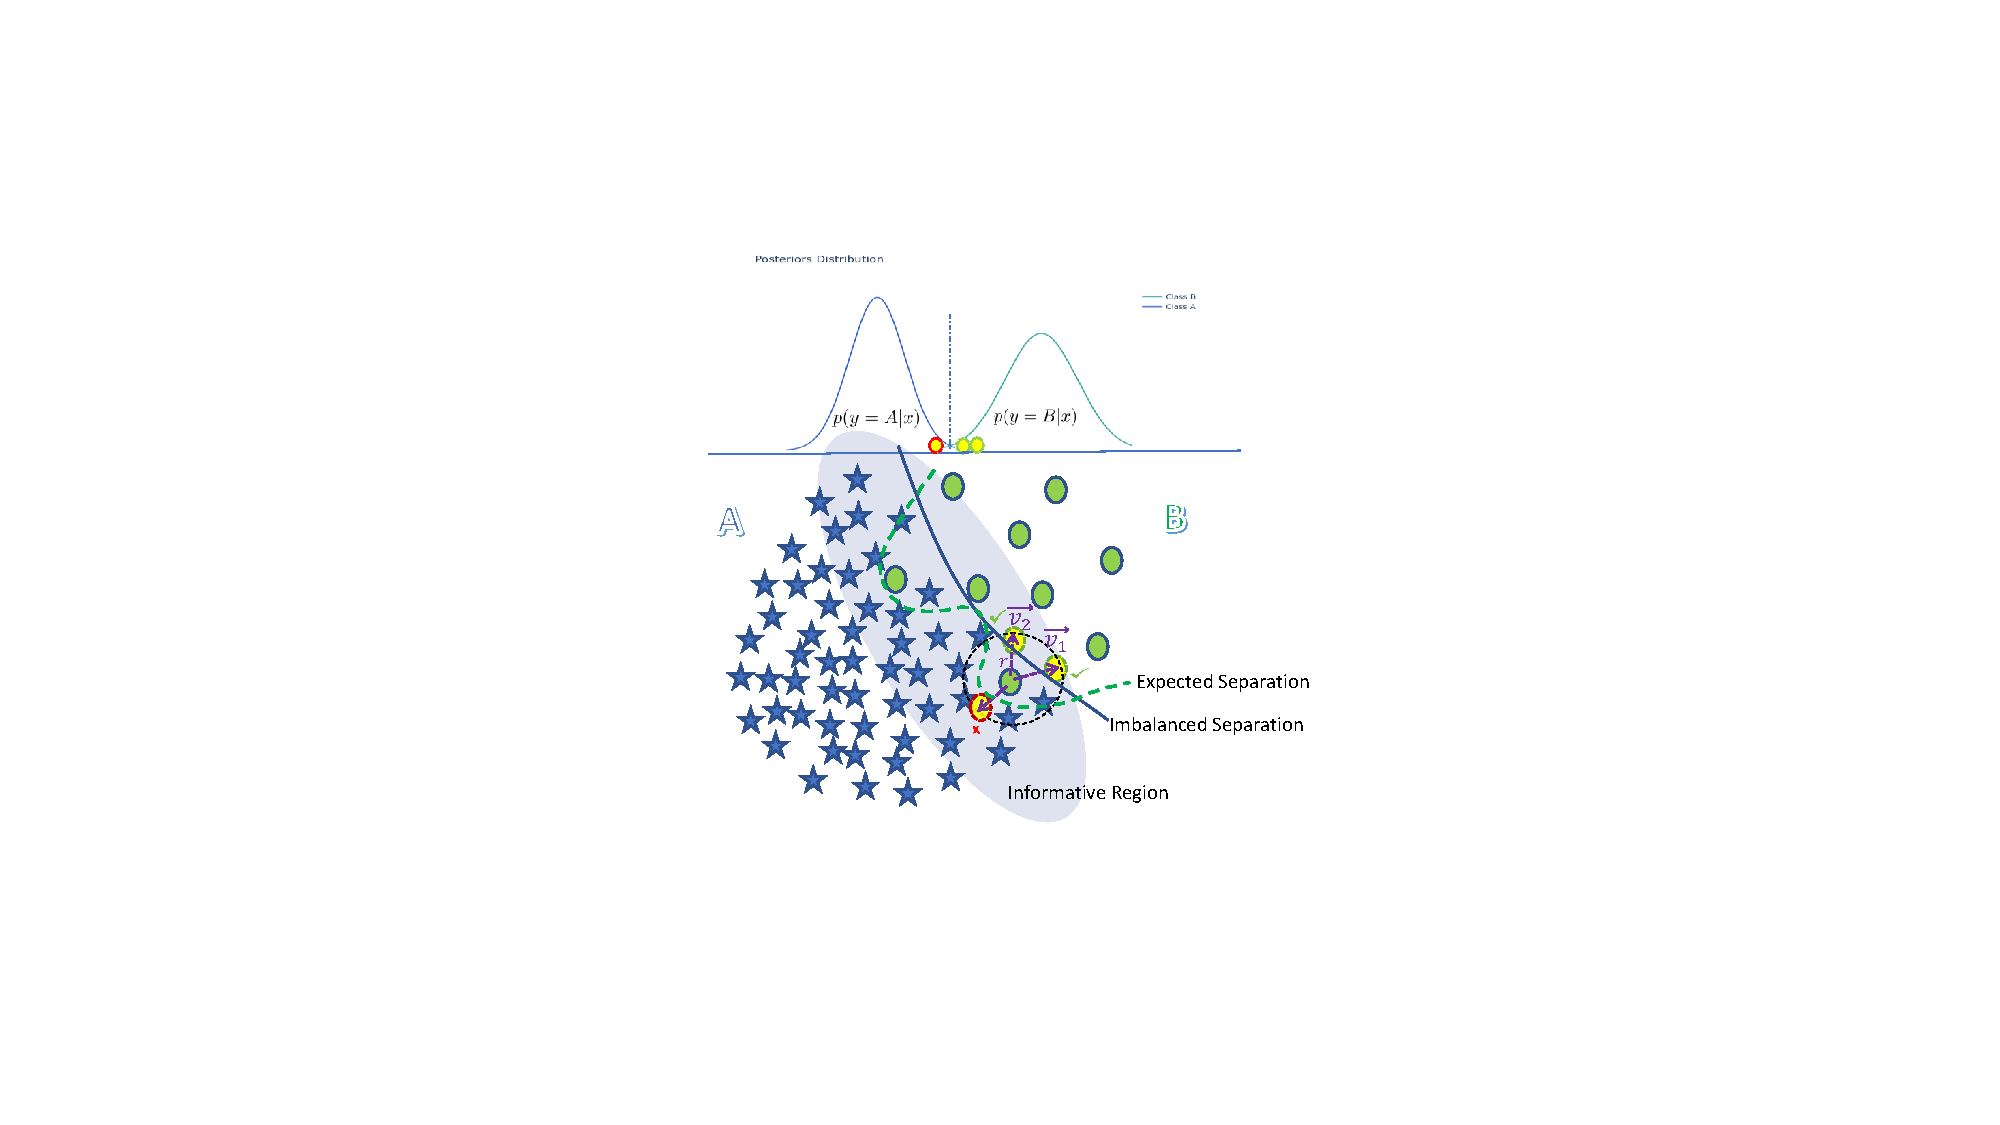
\includegraphics[width=\linewidth, trim=300 150 310 120,clip]{Figures/proplem.pdf}
		\caption{Learning from imbalanced datasets}
		\label{fig:problem}
	\end{figure}
	
	Figure \ref{fig:problem} illustrates our problem on a binary classification. The imbalance in the informative region (light blue eclipse) could lead to separation errors. The dashed green line depicts the expected boundary, while the solid blue line is the model's boundary. Since the minority class is lacking  data in this region, the majority class will dominate the model even with a few noisy samples, and this leads to a shift of the model's boundary. In contrast to the study by Ertekin \textit{et al.} \cite{ertekin_learning_2007} which assumes the informative region is more balanced by nature and proposes a solution that only classifies over the informative samples, our assumption is different. We consider the case that the informative region contains high imbalanced data, which we believe happens in most of the real scenarios. In a more complex setting such as high dimensional and topologically complex data, the problem could be more severe. Therefore, we proposed a technique to tackle the problem of data imbalance by oversampling the minority class in an informative manner. The detail of our proposed technique will be described in Section \ref{sec:method}.         
	
	
	

\section{Methodology}
\label{sec:SIMPOR_method}
To alleviate the negative effects of data imbalance, we propose a comprehensive approach, \MethodnameLong{} (\Methodname), which aims to generate synthetic samples for minority classes. First, the informative region that contains informative samples is determined and balanced by creating surrounding synthetic neighbors for minority samples. The remaining region is then fully balanced by arbitrarily generating minority samples' neighbors. The remainder of this section provides further information about how our approach was developed.  

\subsection{Methodology Motivation}  
As Chazal and Michel mentioned in their work \cite{leroueil_compressibility_1996}, the natural way to highlight the global topological structure of the data is to connect data points' neighbors; our proposed method aligns with their observation by generating surrounding synthetic neighbors for minority samples to preserve data topology. Thus, our technique not only generates more data for minority class but also preserve the underlying topological structure of the entire data. 

Similar to \cite{ertekin_learning_2007} and \cite{aggarwal_active_2020}, we believe that informative samples play the most important role in the prediction success of both traditional machine learning models (e.g., SVM, Naive Bayes) and modern deep learning approaches (e.g., neural network). Thus, our technique finds these informative samples and focuses on augmenting minority data in this region. In this work, an entropy-based active learning strategy mentioned in \ref{sec:EAL} is applied to find the samples that contain more information to the model. This strategy is perhaps the most popular active learning technique and over-performs many other techniques on several datasets \cite{DAL}, \cite{7393573} \cite{settles_analysis_2008}.

\subsection{Generating minority synthetic data}  
\label{sec:solvingOptimization}
\R{1.1a}
\Copy{1.1a}{
A synthetic neighbor $ x'$ and its label $y'$ can be created surrounding a minority sample $x$ by adding a small random vector $v$ to the sample, $x' = x + v$. Thus, $x'$ can be selected on the d-sphere's surface centered at $x$ with a radius of $|\vec{v}|$. For notation convenience, let $r = |\vec{v}|$ be the radius of the d-sphere. To enrich the synthetic samples, $r$ is sampled from a defined Gaussian distribution to generate a new synthetic sample distance each time. This section describes how the direction and distance of a synthetic sample are determined, which can also be represented via the direction and length of vector $\vec{v}$.

It is critical to generate synthetic data in the informative region because synthetic samples can unexpectedly jump across the decision boundary. This can be harmful to models as this might create outliers and reduce the model's performance. Therefore, we safely find vector $\vec{v}$ towards the minority class, such as $\vec{v}_0$ and $\vec{v}_1$ depicted in Figure \ref{fig:problem}.} Our technique is described via a binary classification scenario as follows. 

Let's consider a binary classification problem between majority class A and minority class B. 
From the Bayes' theorem, the posterior probabilities $p(y'=A|x')$ or $p(y'=B|x')$ can be used to present the probabilities that a synthetic sample $x'$ belongs to class A or class B, respectively. Let the two posterior probabilities be $f_0$ and $f_1$; they can be expressed as follows. 
\begin{align}
	\label{eq:posterior}
	p(y'=A|x') = \frac{p(x'|y'=A)\:p(A)}{p(x')} = f_0 \\
	p(y'=B|x') = \frac{p(x'|y'=B)\:p(B)}{p(x')} = f_1  
\end{align}

As mentioned earlier, each synthetic data $x'$ is generated so that it maximizes the probability of $x'$ belonging to the minority class $B$ and minimizes the chance $x'$ falling into the majority class $A$. Thus, a technique that maximizes the fractional posterior $f$ is proposed,   
\begin{align}
	\label{eq:fracpost}
	f &= f_1/f_0  \\
	&=\frac{p(x'|y'=B) \:p(B)}{p(x'|y'=A) \: p(A)}. \label{equ:f_ratio}
\end{align}


\textbf{\textit{Approximation of likelihoods in Equation \ref{equ:f_ratio}:}} A non-parametric kernel density estimates (KDE) is selected to approximate the likelihoods $p(x'|y'=A)$ and $p(x'|y'=B)$ as KDE is flexible and does not require specific assumptions about the data distribution. One can use a parametric statistical model such as Gaussian to approximate the likelihood; however, it oversimplifies the data and does not work effectively with topological complex data, especially in high dimensions. In addition, parametric models require an assumption about the distribution of data which is difficult in real-world problems since we usually do not have such information. On the other hand, KDE only needs a kernel working as a window sliding through the data. Among different commonly used kernels for KDE, we choose Gaussian Kernel as it is a powerful continuous kernel that would also eases the derivative computations for finding optima.
 
\R{PriorApproximation}
\Copy{PriorApproximation}{
\textbf{\textit{Approximation of priors in Equation \ref{equ:f_ratio}:}} Additionally, we estimate the prior probabilities of observing samples in class A ($p(A)$) and class B ($p(B)$) (in Equation \ref{equ:f_ratio}) by the widely-used Empirical Bayes Method \cite{empiricalBayes} to leverage the existing information from the original data. The estimates are denoted as $\widehat{p(A)}$ and $\widehat{p(B)}$ respectively.

\textbf{\textit{Equation \ref{equ:f_ratio} Approximation:} } Let $X_A$ and $X_B$ be the subsets of dataset $X$ which contain samples of class A and class B, $X_A=\{x: y=A  \}$ and $X_B=\{x: y=B  \}$. $N_A$ and $N_B$ are the numbers of samples in $X_A$ and $X_B$. $d$ is the number of data dimensions. $h$ presents the width parameter of the Gaussian kernel. The posterior ratio for each synthetic sample $x'$ then can be estimated as follows:

\begin{align}
	\label{eq:fracpost_estimation}
	f &= \frac{p(x'|y'=B)  \: p(B)}{p(x'|y'=A) \: p(A)} \\
	&\propto \frac{ \frac{1}{N_B h^d} \: \sum_{i=1}^{N_B}{ (2\pi)^{-\frac{d}{2}} \: e^{\frac{1}{2}{(\frac{x'-X_{B_i}}{h})^2} } } \: \widehat{p(B)} }
	{ \frac{1}{N_A h^d} \:  \sum_{j=1}^{N_A}{ (2\pi)^{-\frac{d}{2}} \: e^{ \frac{1}{2} {(\frac{x-X_{A_j}}{h})^2} } }\: \widehat{p(A)} }\\
	& \propto \frac{ \frac{1}{N_B h^d} \: \sum_{i=1}^{N_B}{ \: e^{\frac{1}{2}{(\frac{x'-X_{B_i}}{h})^2} } } \: \widehat{p(B)} }
	{ \frac{1}{N_A h^d} \:  \sum_{j=1}^{N_A}{  \: e^{ \frac{1}{2} {(\frac{x-X_{A_j}}{h})^2} } }\: \widehat{p(A)} }
	\label{equ:f}
\end{align} 
}


\textbf{\textit{Selecting bandwidth parameter $h$ for Gaussian kernel:} } The bandwidth is automatically selected for each dataset using the most common method, namely Scott's rule of thumb, proposed by Scott \cite{scott_2015}. With an attempt to minimize the mean integrated squared error, the parameter is estimated as $h = N^{(-\frac{1}{d+4})}$ where $N$, $d$ are the number of data points and the number of dimensions respectively. This study utilizes a scikitlearn python library for KDE, including bandwidth selection. The implementation detail can be found at \cite{skitlearnKDE}. 

\R{1.1b}
\textbf{\textit{Finding synthetic samples surrounding a minority sample:}} To generate neighbors for each minority sample that maximizes Function \text{f} in Equation \ref{equ:f}, points on each $r$-radius sphere centered at a minority sample are considered synthetic instances. As a result, a vector $\vec{v}$ can be added to a minority sample for generating a new instance. \Copy{1.1b}{The relationship between a synthetic sample $x'$ and a minority sample can be described as follows,
\begin{align}
	\label{equ:vecV}
	\vec{x'} =  \vec{x} + \vec{v},
\end{align}
where the length of $\vec{v}$ is equal to $r$, and $r$ is sampled from a Gaussian distribution,
\begin{align}
     r \sim \mathcal{N}(0,\,(\alpha R)^{2}),
     \label{equ:r_dist}
\end{align}
where $\alpha R$ is the standard deviation of the Gaussian distribution and $ 0< \alpha <=1 $.
The range parameter $R$ is relatively small and computed as the average distance of a minority sample $x$ to its k-nearest neighbors. This will ensure that the generated sample will surround the minority sample. The Gaussian distribution with the mean of zero and the standard deviation $\alpha R$ controls the distance between the synthetic samples and the minority sample. The standard deviation is tuned from 0 to R by a coefficient $\alpha \in (0,1]$. The larger the $\alpha$ is, the farther synthetic data is placed from its original sample.} Consider a minority sample $x$ and its k-nearest neighbors in the Euclidean space, $R$ can be computed as follows:

\begin{align}
	R = \frac{1}{k}\sum\limits_{1}^{k} ||x-x_j ||,
\end{align}
where $||x-x_j||$ is the Euclidean distance between a minority sample $x$ and its $j$th neighbor. $k$ is a parameter indicating selected number of neighbors. 


\begin{figure}[th]
	%[trim=left bottom right top, clip]
	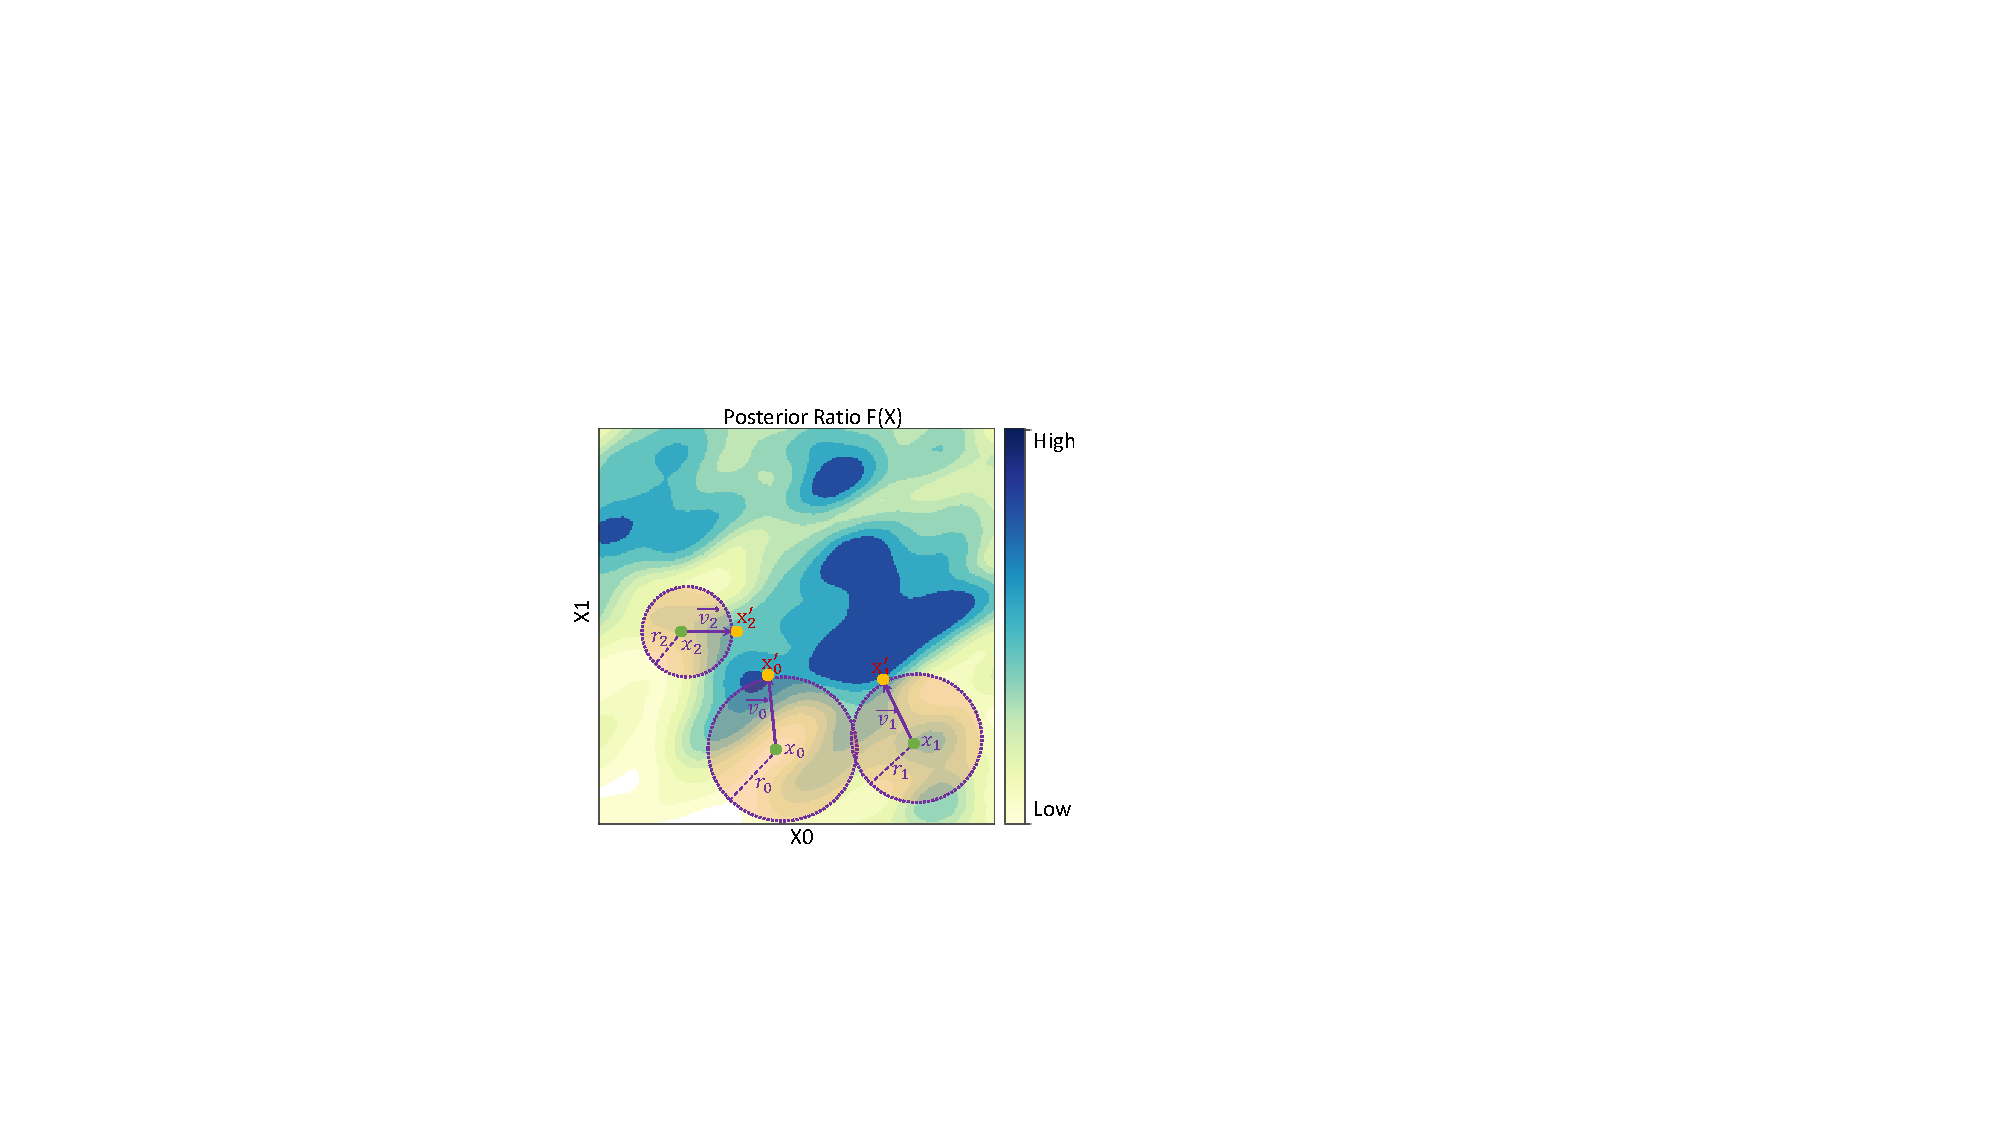
\includegraphics[width=\linewidth, trim=240 120 390 160,clip]{Figures/MaxPosteriorRatio/sphere_maxF.pdf}
	\caption{Demonstration on how \Methodname{} generates three synthetic samples $x'_0, x'_1, x'_2$, from three minority samples $x_0, x_1, x_2$, by maximizing the Posterior Ratio. }
	\label{fig:sphere_maxF}
\end{figure}

Figure \ref{fig:sphere_maxF} depicts a demonstration of finding 3 synthetic samples from 3 minority samples. In practice, one minority can be re-sampled to generate more than one synthetic samples. For a minority sample $x_0$, we find a synthetic sample $x_0'$ by maximizing the objective function $f(x_0'), x_0' \in X$ with a constraint that the Euclidean length of $\vec{v_0}$ equals to a radius $r_0$, $||\vec{v_0}|| = r_0$ or $||\vec{x_0'}-\vec{x_0}||=r_0$ (derived from Equation \ref{equ:vecV}). 


The problem can be described as a constrained optimization problem. For each minority sample $x$, we find a synthetic sample $x'\in \mathbb{R}^d$ lying on the d-sphere centered at $x$ with radius $r$ and maximizing function in Equation \ref{equ:f},
\begin{align}
	\label{prob:optimazation}
	\max_{x'} {f(x')} \;\;\; \textrm{s.t.}\; ||\vec{x'} - \vec{x}||=r.
\end{align}

\textbf{\textit{Solving optimization problem in Equation \ref{prob:optimazation}:}} Interestingly, the problem in Equation\ref{prob:optimazation} can be solved numerically. Function $f(x)$ in Equation \ref{equ:f} is defined and continuous for $x' \in (-\infty, +\infty)$ because all of the exponential components (Gaussian kernels) are continuous and greater than zero. In addition, the constraint, $||\vec{x'} - \vec{x}||=r$, which contains all points on the sphere centered at $x$ with radius $r$ is a closed set (\cite{wikipedia_2021}). Thus, a maximum exits as proved in \cite{maximum_exist}. To enhance the diversity of synthetic data, either the global maximum or any local maximum can be accepted so that the synthetic samples will not simply go to the same direction.  

We solve the problem in Equation \ref{prob:optimazation} by using the Projected Gradient Ascent approach in which we iteratively update the parameter to go up the gradient of the objective function. A local maximum is found if the objective value cannot be increased by any local update. For simplification, we rewrite the problem in Equation \ref{prob:optimazation} by shifting the origin to the considered minority sample. The problem becomes finding the maximum of function $f(x')$, $x' \in \mathbb{R}^d$, constrained on a d-sphere, i.e., $||x'||=r$. Our solution can be described in Algorithm \ref{alg:optimization}. After shifting the coordinates system, we start by sampling a random point on the constraint sphere (line $1-2$). The gradient of the objective function at time $t$, $g_t(x'_t)$, is computed and projected onto the sphere tangent plane as $p_t$ (line $4-5$). It is then normalized and used for update a new $x'_{t+1}$ by rotating a small angle $lr*\theta$ (line $6-7$). The algorithm stops when the value of $f(x')$ is not increased by any update of $x'$. We finally shift to the original coordinates and return the latest $x'_t$.   
\begin{algorithm}[ht]
	\caption{Sphere-Constrained Gradient Ascent for Finding Maximum}
	
	\begin{flushleft}
		\textbf{Input}: A minority sample $x_0$, objective function $f(x,X)$\\
		\textbf{Parameter}: \\
		$r$ : The radius of the sphere centered at $x_0$  \\\
		$\theta$ : Sample space $\theta \in [0,2\pi]$ \\
		$lr$ : Gradient ascent learning rate\\
		
		\textbf{Output}: An local maximum $x'$\\
		\begin{algorithmic}[1]
			\STATE Shift the Origin to $x_0$
			\STATE Randomly initiate $x'_t$ on the sphere with radius $r$	
			\WHILE {converge condition}
			\STATE Compute the gradient at $x'_t$\\
			$g_t(x'_t) = \nabla f(x'_t)$
			\STATE Project the gradient onto the sphere tangent plane\\
			$p_t = g_t - (g_t \cdot x'_t) x_t$
			\STATE Normalize projected vector\\
			$p_t = p_t/ ||p_t||$
			\STATE Update $x'$ on the constrained sphere \\
			$x'_{t+1} = x'_t cos(lr*\theta) + p_t sin (lr*\theta)$ 			
			\ENDWHILE
			\STATE Shift back to the Origin
			\RETURN $x'_t$
		\end{algorithmic}
	\end{flushleft}
	\label{alg:optimization}
\end{algorithm}


\textbf{\textit{Avoiding synthesis of noise:}} To reduce the chance of misplacing synthetic samples on another class region because of noisy borderline and mislabeled minority samples, we set a policy for rejecting minority candidates which are selected for oversampling. The idea is to reject candidates surrounded mainly by other class samples. More specifically, we count the labels of the candidate's $k$-nearest neighbors and reject this candidate if there exists a class that its' number of samples is greater than the number of the minority samples). For example, the candidate is rejected when a class-A sample is selected for generating synthetic data, and its 5-nearest neighbors contain four class-B samples and one class-A sample. This is to avoid selecting mislabeled samples and noisy borderline samples for oversampling.        

\subsection{Algorithm}
Our strategy can be described in Algorithm \ref{alg:SIMPOR}. The algorithm takes an imbalanced dataset as its input and results in a balanced dataset which is a combination of the original dataset and synthetic samples. We first choose an active learning method $AL(\cdot)$ and find a subset of informative samples $S$ by leveraging entropy-based active learning (lines $1-2$). We then generate synthetic data to balance $S$. For each random sample $x_i^c$ in $S$ and belonging to minority class $c$, we randomly sample a small radius $r$ and find a synthetic sample that lies on the sphere centered at $x_i^c$ and maximizes the posterior ratio in Equation \ref{equ:f} (lines $3-11$). The process is repeated until the informative set $S$ is balanced. Similarly, the remaining region is balanced, which can be described in the pseudo-code from line $12$ to line $20$. The final output of the algorithm is a balanced dataset $D'$.       

\begin{algorithm}[ht]
	\caption{\Methodname}
	
	\begin{flushleft}
		\textbf{Input}: Original Imbalance Dataset $D$ including data $X$ and labels $y$.\\
		\textbf{Parameter}: 
		$MA$ is the majority class, $MI$ is a set of other classes.\\
		$k$: Number of  neighbors of the considered sample which determines the maximum range of the sample to its synthetic samples.\\ 
		$\alpha$: preset radius coefficient
		$Count(c, P)$ : A function to count class $c$ sample number in population $P$.\\
		$G(x_0,f,r)$ : Algorithm \ref{alg:optimization}, which returns a synthetic sample on sphere centered at $x_0$ with radius $r$ and maximize Equation \ref{equ:f}.  \\
		\textbf{Output}: Balanced Dataset $D'$ including $\{X',y'\}$
		\begin{algorithmic}[1]
			\STATE Select an Active Learning Algorithm $AL()$
			\STATE Query a subset of informative samples $S \in D$  using $AL$:
			$s  \leftarrow AL(D) $	\\
			
			\COMMENT{Balance the informative region}
			\FOR {$c \in MI$}
			\WHILE {$Count(c, S) \leq Count(MA, S)$ }
			\STATE Select a random $x_i^c \in S$
			\STATE Reject and reselect $x_i^c$ if its label is dominated among k-nearest labels
			\STATE Compute maximum range $R$ based on k-nearest neighbors
			\STATE Randomly sample a radius $r \sim \mathcal{N}(0,\alpha R)$
			\STATE Generate a synthetic neighbor $x'$ from $x_i^c$:
			$x'=G(x_i^c,f,r)$ 
			\STATE Append $x'$ to $D'$
			\ENDWHILE
			\ENDFOR
			
			\COMMENT{Balance the remaining region}
			\FOR {$c$ in $MI$}
			\WHILE { $Count(c, D') \leq Count(MA, D')$ }	
			\STATE Select a random $x_j^c \in \{X-S\}$
			\STATE Compute maximum range $R$ based on $k$
			\STATE Randomly sample a radius $r \sim \mathcal{N}(0,\alpha R)$
			\STATE Generate a synthetic neighbor $x'$ of $x_j^c$ 
			\STATE Append $x'$ to $D'$
			\ENDWHILE
			\ENDFOR
			\RETURN 
		\end{algorithmic}
	\end{flushleft}
	\label{alg:SIMPOR}
\end{algorithm}
	
	

%\section{Algorithm Implementation and Time Complexity}


\section{Algorithm Time Complexity.}
\label{sec:implementation}


\iffalse
Our proposed technique is straightforward in implementation. We first train a neural network model with initial samples and start querying the next batches of data based on the entropy scores from the previous model to find informative samples. The model is then updated with new batches of data until the entropy scores reach a certain threshold. All the informative samples are then balanced first, and the remaining data are balanced later. Each synthetic data point is generated by finding local maxima in Equation \ref{equ:f}.
\fi

The costly part of \Methodname{} is that each synthetic sample requires computing a kernel density estimation of the entire dataset. Elaborately, let $n$ be the number of samples of the dataset. In the worst case, the numbers of samples of minority and majority class are $N_B = 1$ and $N_A = n-1$, respectively. We need to generate $n-2$ synthetic samples to balance the dataset completely. Since each generated sample must loop through the entire dataset of size $n$ to estimate the density, the algorithm complexity is $O(n^2)$. 

Although generating synthetic data is only a one-time process, and this does not affect the classification efficiency in the testing phase, we still try to alleviate its weakness by providing parallelized implementations to reduce the time complexity to $O(n)$. Specifically, each exponential component in Equation \ref{equ:f} is computed parallelly, utilizing GPU or CPU threads. Ellaborately, Equation \ref{equ:f} can be rewritten as $N_B$ components of $e^{\frac{1}{2} (\frac {x - X_{B_i}}{h})^2}$ and $N_A$ components of $e^{\frac{1}{2} (\frac {x - X_{A_i}}{h})^2}$. Fortunately, they are all independent and can be processed parallelly. Thus, with a sufficient hardware resource, the consumption time for the kernel density estimation of each synthetic data point is then reduced by $N_A+N_B=n$ times, which significantly simplifies the complexity to $O(n)$.


	
	


\section{Experiments}
\label{sec:experiments}
\R{sow}
\Copy{sow}{
In this section, we explore the techniques via binary classification problems on an artificial dataset (i.e., Moon) and 41 real-world datasets (i.e., KEEL, UCI, Credit Card Fraud) with a diversity of imbalance ratios and different numbers of features. Samples in Moon have two features, while other datasets contain various numbers of features and imbalance ratios.} Dataset details are described in Table \ref{tab:dataDecription}.  
The implementation steps to balance datasets follow Algorithm \ref{alg:SIMPOR}. To evaluate our proposed balancing technique, we compare the classification performance to different widely-used and state-of-the-art techniques. More specifically, We compare \Methodname{} to SMOTE \cite{chawla_smote:_2002}, Borderline-SMOTE \cite{bordersmote},  ADASYN \cite{ADASYN}, DeepSMOTE \cite{deepsmote}, Gaussian Distribution Based Oversampling (GDO) \cite{bib:GDO}, SVMCS \cite{cssvm}, EE \cite{EE}. To evaluate the classifications performance for skewed datasets, we measure widely-used metrics, i.e., F1-score and Area Under The Curve (AUC). 

% Table generated by Excel2LaTeX from sheet 'KEEL Data Description'
\Copy{datasetTable}{
\begin{table}[htbp]
	\centering
	\caption{Dataset Description.}
	
	\begin{tabular}{lccc}
		\hline
		dataset & \#samples & \#features & IR \bigstrut\\
		\hline
		glass1 & 214   & 9     & 1.8 (138:76)\bigstrut[t]\\
		wisconsin & 683   & 9     & 1.9 (444:239) \\
		pima  & 768   & 8     & 1.9 (500:268)\\
		glass0 & 214   & 9     & 2.1 (144:70) \\
		yeast1 & 1484  & 8     & 2.5 (1055:429)\\
		haberman & 306   & 3     & 2.8 (225:81) \\
		vehicle1 & 846   & 18    & 2.9 (629:217)\\
		vehicle2 & 846   & 18    & 2.9 (628:218)\\
		vehicle3 & 846   & 18    & 3.0 (634:212)\\
		creditcard & 1968  & 30    & 3.0 (1476:492)\\
		glass-0-1-2-3\_vs\_4-5-6 & 214   & 9     & 3.2 (163:51)\\
		vehicle0 & 846   & 18    & 3.3 (647:199)\\
		ecoli1 & 336   & 7     & 3.4 (259:77)\\
		new-thyroid1 & 215   & 5     & 5.1 (180:35) \\
		new-thyroid2 & 215   & 5     & 5.1 (180:35)\\
		ecoli2 & 336   & 7     & 5.5 (284:52)\\
		glass6 & 214   & 9     & 6.4 (185:29)\\
		yeast3 & 1484  & 8     & 8.1 (1321:63)\\
		ecoli3 & 336   & 7     & 8.6 (301:35)\\
		page-blocks0 & 5472  & 10    & 8.8 (4913:559)\\
		yeast-2\_vs\_4 & 514   & 8     & 9.0 (463:51)\\
		yeast-0-5-6-7-9\_vs\_4 & 528   & 8     & 9.4 (477:51)\\
		vowel0 & 988   & 13    & 10.0 (898:90)\\
		glass-0-1-6\_vs\_2 & 192   & 9     & 10.3 (175:17)\\
		glass2 & 214   & 9     & 11.6 (197:17)\\
		yeast-1\_vs\_7 & 459   & 7     & 14.3 (429:30)\\
		glass4 & 214   & 9     & 15.5 (201:13)\\
		ecoli4 & 336   & 7     & 15.8 (316:20)\\
		page-blocks-1-3\_vs\_4 & 472   & 10    & 15.9 (444:28)\\
		abalone9-18 & 731   & 8     & 16.4 (689:42)\\
		yeast-1-4-5-8\_vs\_7 & 693   & 8     & 22.1 (663:30)\\
		glass5 & 214   & 9     & 22.8 (205:9)\\
		yeast-2\_vs\_8 & 482   & 8     & 23.1 (462:20)\\
		car\_eval\_4 & 1728  & 21    & 25.6 (1663:65)\\
		wine\_quality & 4898  & 11    & 25.8 (4715:183)\\
		yeast\_me2 & 1484  & 8     & 28.0 (1433:51)\\
		yeast4 & 1484  & 8     & 28.1 (1433:51)\\
		yeast-1-2-8-9\_vs\_7 & 947   & 8     & 30.6 (917:30)\\
		yeast5 & 1484  & 8     & 32.7 (1440:44)\\
		yeast6 & 1484  & 8     & 41.4 (1449:35)\\
		abalone19 & 4174  & 8     & 129.4 (689:42)\\
	\end{tabular}%
	\label{tab:dataDecription}%
\end{table}%
}


\subsection{Implementation Detail}
This section describes the general settings and implementation details for the experimental techniques. Our implementation code is publicly available on Github \footnote{\url{https://github.com/nsh135/_SIMPOR_}}.  


\subsubsection{\Methodname{} settings}
\Copy{ALImplementation}{
In order to find the informative subset, we leverage entropy-based active learning. We first utilize a neural network model playing a role as a classifier to find high-entropy samples (Note that the classifier for finding the informative subset differs from the classifiers for the final classification evaluation after all balancing techniques are applied to the data). The detailed steps are introduced in Section \ref{sec:EAL}. The model contains two fully connected hidden layers with \textit{relu} activation functions and 10 neurons in each layer. The output layer applies the soft-max activation function. The model is trained in a maximum of 300 epochs with an early stop option when the loss is not significantly improved after updating weights. The model is trained firstly on a random set of three samples each class (six samples two classes). This model is then used to estimate entropy scores for the remaining data. We then select next 20  highest entropy samples ($k$=20) for the next informative data batch. This batch is concatenated to the initial batch for updating the classifiers and accumulated to the informative set. The steps are repeated until the informative set reaches desire informative portion (IP). In these experiments, we set IP=0.3 corresponding to 30 percent of the training size selected for the informative set. 
}

To solve the optimization problem in Equation \ref{prob:optimazation} for finding optima (this differs from the classification optimization for the evaluation) introduced in Section \ref{sec:solvingOptimization}, we use a gradient ascent method with the gradient rate of $1e-5$ and the maximum iteration of 300.   

\subsubsection{Evaluation Classification settings}
Considering each imbalanced dataset as a classification problem, we use the classification testing performance for the technique comparison. Each dataset is randomly split into two parts, 80\% for training and 20\% for testing. The classifiers are trained on training sets after applying the techniques. The results are reported on the raw testing sets (There isn't any technique applied on the testing sets; thus, they are also possibly class imbalanced). We use F1-score and AUC for the evaluation metrics as they are suitable and widely used to evaluate imbalanced data. Reported testing results for each dataset are the averages of 5 experimental trials.

The classifiers are constructed by neural networks with the input and output sizes corresponding to the number of datasets' features and unique labels. We use the same classifier structure (number of hidden layers, number of neurons in each layer, learning rate, optimizer) for all compared datasets. The detail of neural network implementation is described in Table \ref{tab:model_setting}. 
For baseline technique settings, we follow the experimental parameter sets in \cite{bib:GDO} as we share very similar datasets and comparison techniques. For DeepSMOTE settings, the DCGAN input and output sizes are modified to adapt with each dataset, while other settings is taken from the initial parameter set in \cite{deepsmote}.


\begin{table}[htbp!]
	\centering
	\caption{Classification models' setting for each dataset.}
	%\rule{\linewidth}{3cm}
	\label{tab:model_setting}
	\resizebox{0.9\columnwidth}{!}{%
	
\begin{tabular}{lp{29.57em}}
	\toprule
	Method & \multicolumn{1}{l}{Parameter} \\
	\midrule
	SIMPOR & \multicolumn{1}{l}{k\_neighbors=5, r\_distribtuion=Gaussian, IP=0.3} \\
	GDO   & \multicolumn{1}{l}{k\_neighbors=5, d=1} \\
	SMOTE & \multicolumn{1}{l}{k\_neighbors=5, sampling\_strategy=`auto',random\_state=None} \\
	BL-SMOTE & \multicolumn{1}{l}{k\_neighbors=5, sampling\_strategy=`auto', random\_state=None} \\
	ADASYN & \multicolumn{1}{l}{k\_neighbors=5, sampling\_strategy=`auto', random\_state=None} \\
	EE    & \multicolumn{1}{l}{\#estimators=10, Estimater=AdaBoostClassifier} \\
	DeepSMOTE   & \multicolumn{1}{l}{Sigma=1, Lambda=0.1} \\
	\midrule
	Classifier & \multicolumn{1}{l}{Parameter} \\
	\midrule
	Architecture & \multicolumn{1}{l}{neuron/layer=100, \#layers=3} \\
	Optimization & optimizer=`adam',  epochs=200, batch\_size=32, learning\_rate=0.1, reduce\_lr\_loss(factor=0.9,epsilon=1e-4,patience=5) \\
	\bottomrule
\end{tabular}%

	}
\end{table}%


\subsection{\Methodname{} on artificial Moon dataset}

\begin{figure}[h!]	
	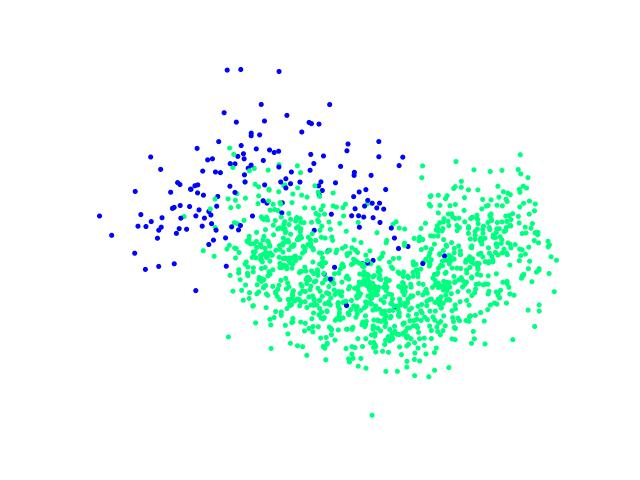
\includegraphics[width=0.9\linewidth]{Figures/moon/ImbalancedData}
	\caption{Artificial class imbalanced Moon dataset with IR of 7:1.}
	\label{fig:raw_moon}
\end{figure}


\begin{figure*}[th]
	\centering
	%[trim=left bottom right top, clip]
	\begin{subfigure}[]{0.3\linewidth}
		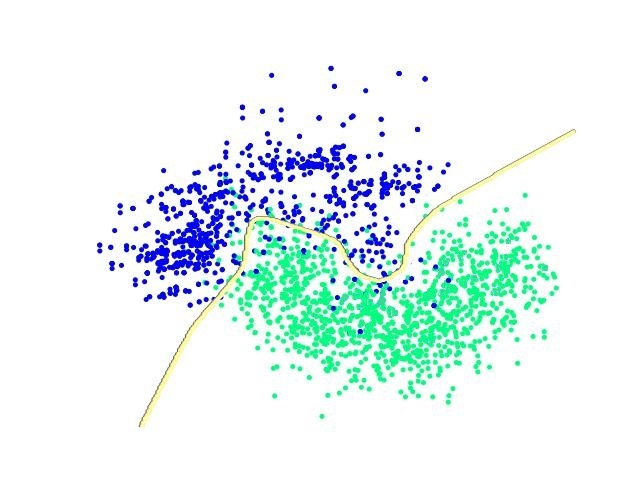
\includegraphics[width=\linewidth]{Figures/moon/Training_Data_PLot_SIMPOR}
		\caption{\Methodname{}.}
		\label{fig:simpor_moon}
	\end{subfigure}
	\hspace{0.1em}% 
	\begin{subfigure}[]{0.3\linewidth}
		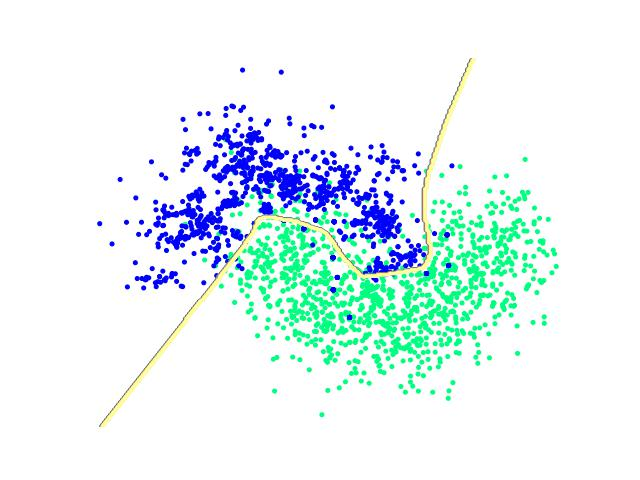
\includegraphics[width=\linewidth]{Figures/moon/Training_Data_PLot_GDO}
		\caption{GDO.}
		\label{fig:gdo_moon}
	\end{subfigure}
	\hspace{0.1em}% 
	\begin{subfigure}[]{0.3\linewidth}
		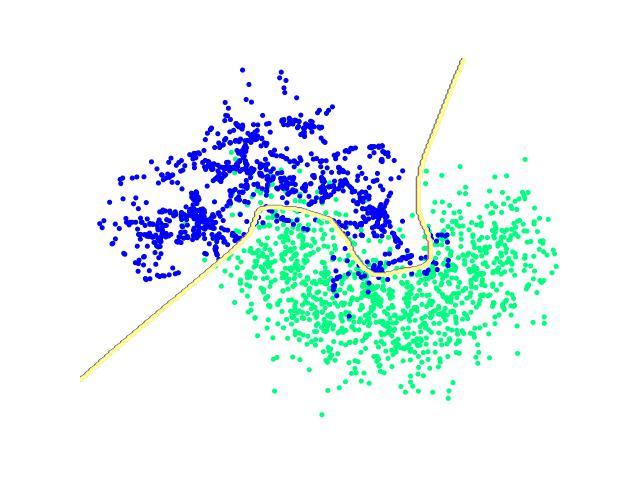
\includegraphics[width=\linewidth]{Figures/moon/Training_Data_PLot_SMOTE}
		\caption{SMOTE.}
		\label{fig:smote_moon}
	\end{subfigure}
	\\
	\begin{subfigure}[]{0.3\linewidth}
		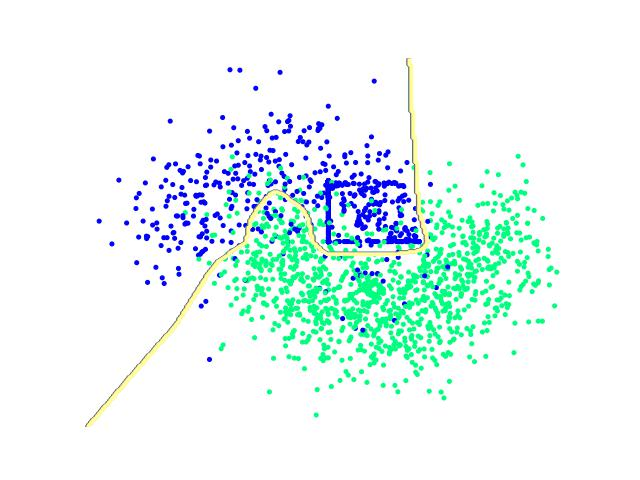
\includegraphics[width=\linewidth]{Figures/moon/Training_Data_PLot_DeepSMOTE}
		\caption{ DeepSMOTE.}
		\label{fig:deepsmote_moon}
	\end{subfigure}
	\hspace{0.1em}% 
	\begin{subfigure}[]{0.3\linewidth}
		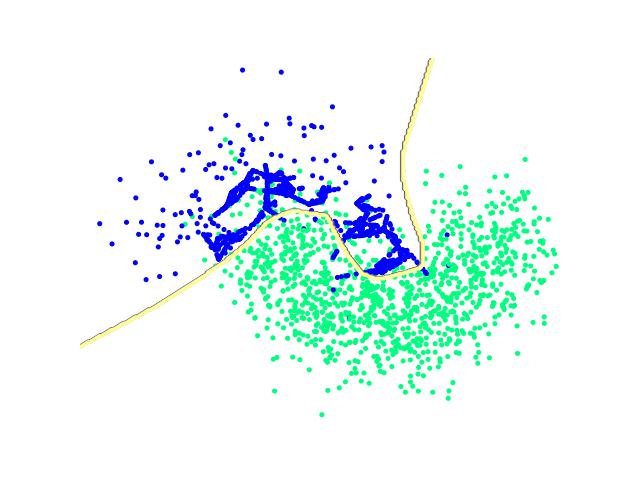
\includegraphics[width=\linewidth]{Figures/moon/Training_Data_PLot_BorderlineSMOTE}
		\caption{BorderlineSMOTE.}
		\label{fig:border_smote_moon}
	\end{subfigure}
	\hspace{0.1em}% 
	\begin{subfigure}[]{0.3\linewidth}
		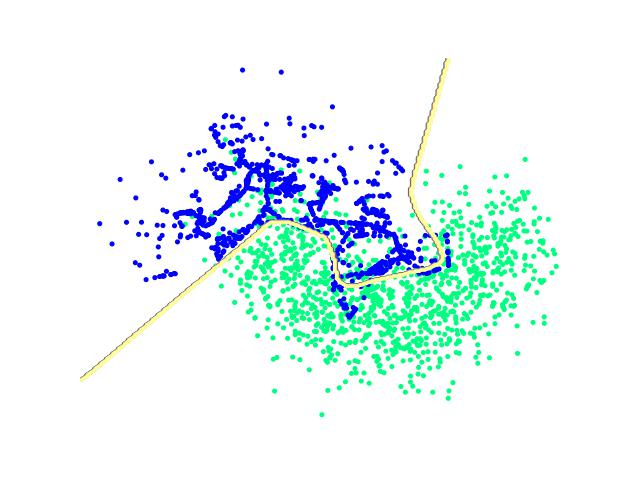
\includegraphics[width=\linewidth]{Figures/moon/Training_Data_PLot_ADASYN}
		\caption{ADASYN. }
		\label{fig:adasyn_moon}
	\end{subfigure}
	
	\caption{Data plot and model's decision boundary visualization for Moon Dataset over different techniques.}
	\label{fig:MoonResults}
\end{figure*}

\Copy{moonGeneration}{
We implement techniques on an artificial 2-dimension dataset for demonstration purposes. We first generate the balanced synthetic MOON dataset using python library \textit{sklearn.datasets.make\_moons}. The generated MOON contains 3000 samples labeled in two classes, and each instance has two numerical features with values ranging from 0 to 1. We then make the dataset artificially imbalanced with an Imbalance Ratio of 7:1 by randomly removing 1285 samples from one class.} As a result, the training dataset becomes imbalanced, as visualized in Figure \ref{fig:raw_moon}.

Figure \ref{fig:MoonResults} captures the classification for different techniques. We also visualize the model decision boundaries to provide additional information on how the classification models are affected. We use a fully connected neural network described in Table \ref{tab:model_setting} to classify the data.




% Table generated by Excel2LaTeX from sheet 'Accuracy'
\begin{table}[htbp!]
	\centering
	\caption{Classification Result on Moon Dataset.}
	\resizebox{\columnwidth}{!}{%
		
	\begin{tabular}{crcccccc}
		Metric &       & SIMPOR & SMOTE & BL-SMOTE & DeepSMOTE   & ADASYN & GDO \bigstrut[b]\\
		\hline
		F1-score &       & 0.883 & 0.824 & 0.827 & 0.842 & 0.785 & 0.817 \bigstrut[t]\\
		AUC   &       & 0.961 & 0.957 & 0.955 & 0.959 & 0.955 & 0.959 \\
	\end{tabular}%

}
	\label{tab:MoonPerformance}
\end{table}%

\subsubsection{Results and Discussion}
From the visualization shown in Figure \ref{fig:MoonResults} and the classification performance results in Table \ref{tab:MoonPerformance}, it is clear that \Methodname{} performs better than others by up to 10\% on F1-score and 1.1\% on AUC. We can see that DeepSMOTE (DeepSM) creates dense squared noise and pushes the decision boundary to the majority class. Due to the fact that SMOTE-based methods does not take the informative region into account, unbalanced data in this area lead to a severe error in decision boundary. In Figures \ref{fig:adasyn_moon} and \ref{fig:border_smote_moon}, BorderlineSMOTE (BL-SMOTE) and ADASYN focus on the area near the model's decision boundary, but they inherit a drawback from SMOTE; any noise or mislabeled samples can, unfortunately, create very dense bridges crossing the expected border and lead to decision errors. Figure \ref{fig:gdo_moon} shows that GDO also generates local gaussian groups of samples near the boder and thus create errors. This phenomenon might cause by a few mis-labeled sample points. In contrast, by generating neighbors of minority samples in the direction towards the minority class and balancing the informative region, \Methodname{} (Figure \ref{fig:simpor_moon}) helps the classifier to make a better decision with a solid smooth decision boundary. Poorly-placed synthetic samples are significantly less than that of others. 


\subsection{\Methodname{} on forty-one real datasets}
\label{subsec:41Datasets}
\Copy{datasetDetail}{
In this section, we compare the proposed technique on 41 real two-class datasets with a variable number of features and Imbalance Ratios, i.e., KEEL datasets \cite{ KEEL_detail,KEEL_dataset}, UCI datasets fetched from Sklearn tool \cite{imbalancedlearnFetch_datasetsx2014, uci_imbalance_dataset} and Credit Card Fraud \cite{kaggleCreditCard} dataset. Since the original Credit Card Fraud contains a large number of banking normal and fraud transaction samples (284,807) which significantly reduces our experimental efficiency, we reduced the dataset size by randomly removing normal class transactions to reach an imbalance ratio of 3.0. Other datasets are kept as their original versions after removing bad samples (containing Null values). The datasets are described in Table \ref{tab:dataDecription}. 
}
\subsubsection{Classification results}
\label{sec:classificationResult}
% Table generated by Excel2LaTeX from sheet 'MacroF1'

\begin{table}[!htbp]
	\centering
	\caption{F1-score over different datasets.}
	\resizebox{0.97\columnwidth}{!}{%
	
  \begin{tabular}{lrrrrrrrr}
  	\toprule
  	& \multicolumn{1}{c}{SIMPOR} & \multicolumn{1}{c}{GDO} & \multicolumn{1}{c}{SMOTE} & \multicolumn{1}{c}{BL-SMOTE} & \multicolumn{1}{c}{ADASYN} & \multicolumn{1}{c}{DeepSM} & \multicolumn{1}{c}{SVMCS} & \multicolumn{1}{c}{EE} \\
  	\midrule
  	glass1 & 0.729 & \textbf{0.741} & 0.707 & 0.729 & 0.729 & 0.706 & 0.719 & 0.705 \\
  	wisconsin & \textbf{0.962} & 0.959 & 0.953 & 0.958 & 0.956 & 0.960 & 0.958 & 0.957 \\
  	pima  & \textbf{0.777} & 0.699 & 0.714 & 0.720 & 0.700 & 0.721 & 0.742 & 0.731 \\
  	glass0 & \textbf{0.840} & 0.799 & 0.804 & 0.795 & 0.806 & 0.813 & 0.835 & 0.811 \\
  	yeast1 & \textbf{0.715} & 0.676 & 0.675 & 0.685 & 0.672 & 0.673 & 0.685 & 0.678 \\
  	haberman & \textbf{0.601} & 0.599 & 0.589 & 0.587 & 0.580 & 0.587 & 0.586 & 0.584 \\
  	vehicle1 & \textbf{0.824} & 0.815 & 0.807 & 0.796 & 0.817 & 0.785 & 0.784 & 0.808 \\
  	vehicle2 & \textbf{0.987} & 0.967 & 0.977 & 0.978 & 0.981 & 0.954 & 0.976 & 0.981 \\
  	vehicle3 & \textbf{0.821} & 0.766 & 0.785 & 0.792 & 0.806 & 0.780 & 0.782 & 0.785 \\
  	creditcard & \textbf{0.954} & 0.935 & 0.946 & 0.944 & 0.943 & 0.947 & 0.907 & 0.939 \\
  	glass-0-1-2-3\_vs\_4-5-6 & 0.850 & 0.923 & 0.918 & 0.912 & 0.915 & \textbf{0.929} & 0.907 & 0.905 \\
  	vehicle0 & 0.933 & 0.956 & \textbf{0.970} & 0.965 & 0.965 & 0.952 & \textbf{0.970} & 0.969 \\
  	ecoli1 & 0.831 & 0.822 & 0.838 & 0.818 & 0.815 & \textbf{0.853} & 0.824 & 0.827 \\
  	new-thyroid1 & 0.970 & \textbf{0.979} & 0.946 & 0.953 & 0.953 & 0.902 & 0.946 & 0.946 \\
  	new-thyroid2 & 0.962 & \textbf{0.982} & 0.938 & 0.938 & 0.938 & 0.872 & 0.930 & 0.930 \\
  	ecoli2 & \textbf{0.922} & 0.880 & 0.905 & 0.864 & 0.884 & 0.887 & 0.909 & 0.914 \\
  	glass6 & \textbf{0.952} & 0.899 & 0.875 & 0.880 & 0.869 & 0.864 & 0.880 & 0.880 \\
  	yeast3 & 0.862 & 0.818 & 0.842 & 0.836 & 0.829 & 0.831 & 0.867 & \textbf{0.879} \\
  	ecoli3 & 0.806 & 0.791 & 0.790 & 0.792 & 0.792 & \textbf{0.829} & 0.827 & 0.824 \\
  	page-blocks0 & \textbf{0.926} & 0.904 & 0.909 & 0.900 & 0.900 & 0.913 & 0.919 & 0.912 \\
  	yeast-2\_vs\_4 & 0.883 & 0.875 & \textbf{0.893} & 0.844 & 0.866 & 0.817 & 0.807 & 0.772 \\
  	yeast-0-5-6-7-9\_vs\_4 & \textbf{0.824} & 0.752 & 0.754 & 0.781 & 0.758 & 0.747 & 0.813 & 0.805 \\
  	vowel0 & \textbf{1.000} & \textbf{1.000} & \textbf{1.000} & \textbf{1.000} & \textbf{1.000} & 0.997 & \textbf{1.000} & 0.997 \\
  	glass-0-1-6\_vs\_2 & \textbf{0.771} & 0.692 & 0.733 & 0.725 & 0.707 & 0.524 & 0.685 & 0.646 \\
  	glass2 & 0.737 & 0.717 & \textbf{0.839} & 0.805 & 0.801 & 0.779 & 0.701 & 0.666 \\
  	yeast-1\_vs\_7 & \textbf{0.710} & 0.663 & 0.595 & 0.654 & 0.608 & 0.614 & 0.681 & 0.691 \\
  	glass4 & 0.795 & 0.871 & 0.846 & 0.850 & 0.859 & \textbf{0.892} & 0.811 & 0.819 \\
  	ecoli4 & \textbf{0.909} & 0.841 & 0.893 & 0.883 & 0.883 & 0.863 & 0.893 & 0.893 \\
  	page-blocks-1-3\_vs\_4 & 0.982 & 0.944 & 0.964 & 0.972 & 0.964 & 0.982 & \textbf{0.990} & \textbf{0.990} \\
  	abalone9-18 & 0.777 & 0.763 & 0.760 & 0.767 & 0.773 & 0.752 & \textbf{0.817} & 0.792 \\
  	yeast-1-4-5-8\_vs\_7 & 0.593 & \textbf{0.637} & 0.584 & 0.618 & 0.628 & 0.487 & 0.489 & 0.489 \\
  	glass5 & 0.912 & 0.843 & 0.792 & \textbf{0.919} & 0.780 & 0.792 & 0.633 & 0.633 \\
  	yeast-2\_vs\_8 & \textbf{0.884} & 0.758 & 0.746 & 0.772 & 0.750 & 0.823 & 0.876 & 0.876 \\
  	car\_eval\_4 & \textbf{1.000} & 0.967 & 0.997 & 0.994 & 0.997 & 0.993 & \textbf{1.000} & \textbf{1.000} \\
  	wine\_quality & \textbf{0.753} & 0.681 & 0.660 & 0.690 & 0.674 & 0.669 & 0.675 & 0.674 \\
  	yeast\_me2 & 0.701 & 0.638 & 0.668 & 0.655 & 0.656 & 0.690 & \textbf{0.707} & 0.702 \\
  	yeast4 & \textbf{0.793} & 0.698 & 0.682 & 0.690 & 0.671 & 0.738 & 0.752 & 0.752 \\
  	yeast-1-2-8-9\_vs\_7 & \textbf{0.775} & 0.642 & 0.612 & 0.633 & 0.607 & 0.698 & 0.750 & 0.750 \\
  	yeast5 & 0.667 & 0.854 & 0.871 & 0.877 & \textbf{0.881} & 0.786 & 0.839 & 0.844 \\
  	yeast6 & \textbf{0.745} & 0.734 & 0.730 & 0.724 & 0.705 & 0.696 & 0.708 & 0.738 \\
  	abalone19 & 0.498 & 0.500 & \textbf{0.526} & 0.518 & 0.524 & 0.497 & 0.498 & 0.498 \\
  	\bottomrule
  \end{tabular}%
	}
	\label{tab:F1AllDatasets}%
\end{table}%

% Table generated by Excel2LaTeX from sheet 'MicroGmean'
\begin{table}[!htbp]
	\centering
	\caption{AUC result over different datasets.}
	\resizebox{0.97\columnwidth}{!}{%
		
     \begin{tabular}{lrrrrrrrr}
 	\toprule
 	& \multicolumn{1}{c}{SIMPOR} & \multicolumn{1}{c}{GDO} & \multicolumn{1}{c}{SMOTE} & \multicolumn{1}{c}{BL-SMOTE} & \multicolumn{1}{c}{ADASYN} & \multicolumn{1}{c}{DeepSM} & \multicolumn{1}{c}{SVMCS} & \multicolumn{1}{c}{EE} \\
 	\midrule
 	glass1 & 0.798 & \textbf{0.818} & 0.788 & 0.782 & 0.807 & 0.804 & 0.800 & 0.795 \\
 	wisconsin & \textbf{0.995} & 0.992 & 0.992 & 0.992 & 0.992 & 0.991 & \textbf{0.995} & 0.994 \\
 	pima  & \textbf{0.858} & 0.790 & 0.800 & 0.804 & 0.782 & 0.810 & 0.826 & 0.818 \\
 	glass0 & \textbf{0.901} & 0.879 & 0.885 & 0.859 & 0.873 & 0.891 & 0.896 & 0.882 \\
 	yeast1 & \textbf{0.811} & 0.758 & 0.753 & 0.753 & 0.746 & 0.776 & 0.782 & 0.774 \\
 	haberman & 0.675 & 0.662 & 0.660 & 0.673 & 0.667 & 0.686 & 0.686 & \textbf{0.689} \\
 	vehicle1 & \textbf{0.936} & 0.917 & 0.922 & 0.920 & 0.929 & 0.924 & 0.920 & 0.928 \\
 	vehicle2 & \textbf{0.999} & 0.998 & \textbf{0.999} & \textbf{0.999} & \textbf{0.999} & 0.991 & \textbf{0.999} & \textbf{0.999} \\
 	vehicle3 & \textbf{0.918} & 0.871 & 0.895 & 0.897 & 0.900 & 0.901 & 0.903 & 0.904 \\
 	creditcard & \textbf{0.974} & 0.969 & 0.966 & 0.962 & 0.962 & 0.961 & 0.968 & 0.945 \\
 	glass-0-1-2-3\_vs\_4-5-6 & 0.968 & 0.987 & \textbf{0.989} & 0.976 & 0.988 & 0.987 & 0.985 & 0.985 \\
 	vehicle0 & 0.975 & 0.991 & 0.995 & 0.995 & \textbf{0.996} & 0.992 & 0.995 & \textbf{0.996} \\
 	ecoli1 & 0.949 & 0.948 & \textbf{0.952} & 0.942 & 0.943 & 0.951 & 0.951 & 0.950 \\
 	new-thyroid1 & \textbf{0.999} & \textbf{0.999} & 0.997 & 0.997 & 0.997 & 0.982 & 0.997 & 0.997 \\
 	new-thyroid2 & \textbf{0.999} & \textbf{0.999} & 0.998 & 0.998 & 0.997 & 0.977 & 0.998 & \textbf{0.999} \\
 	ecoli2 & 0.950 & 0.953 & 0.957 & 0.946 & 0.958 & 0.957 & 0.959 & \textbf{0.960} \\
 	glass6 & \textbf{0.963} & 0.960 & 0.920 & 0.833 & 0.841 & 0.894 & 0.939 & 0.877 \\
 	yeast3 & \textbf{0.968} & 0.943 & 0.935 & 0.927 & 0.937 & 0.946 & 0.966 & 0.967 \\
 	ecoli3 & 0.883 & 0.879 & 0.878 & 0.880 & 0.883 & 0.891 & \textbf{0.897} & 0.885 \\
 	page-blocks0 & \textbf{0.990} & 0.986 & 0.969 & 0.982 & 0.984 & 0.981 & 0.986 & 0.986 \\
 	yeast-2\_vs\_4 & 0.974 & \textbf{0.976} & 0.961 & 0.959 & 0.960 & 0.907 & 0.972 & 0.949 \\
 	yeast-0-5-6-7-9\_vs\_4 & 0.915 & \textbf{0.923} & 0.881 & 0.904 & 0.866 & 0.876 & 0.918 & 0.914 \\
 	vowel0 & \textbf{1.000} & \textbf{1.000} & \textbf{1.000} & \textbf{1.000} & \textbf{1.000} & \textbf{1.000} & \textbf{1.000} & \textbf{1.000} \\
 	glass-0-1-6\_vs\_2 & \textbf{0.942} & 0.897 & 0.905 & 0.892 & 0.910 & 0.886 & 0.907 & 0.941 \\
 	glass2 & 0.929 & 0.917 & 0.923 & 0.923 & \textbf{0.952} & 0.919 & 0.940 & 0.932 \\
 	yeast-1\_vs\_7 & \textbf{0.848} & 0.777 & 0.677 & 0.761 & 0.685 & 0.702 & 0.791 & 0.795 \\
 	glass4 & 0.955 & 0.976 & 0.954 & \textbf{0.987} & 0.949 & 0.979 & 0.972 & 0.975 \\
 	ecoli4 & \textbf{0.997} & 0.978 & 0.984 & 0.984 & 0.989 & 0.953 & 0.990 & 0.988 \\
 	page-blocks-1-3\_vs\_4 & \textbf{1.000} & 0.997 & 0.999 & 0.999 & 0.999 & 0.999 & 0.999 & 0.999 \\
 	abalone9-18 & 0.934 & 0.920 & 0.933 & 0.929 & 0.919 & 0.898 & 0.930 & \textbf{0.940} \\
 	yeast-1-4-5-8\_vs\_7 & \textbf{0.823} & 0.746 & 0.721 & 0.734 & 0.721 & 0.721 & 0.769 & 0.754 \\
 	glass5 & 0.987 & \textbf{0.990} & 0.985 & 0.983 & 0.987 & 0.987 & \textbf{0.990} & 0.988 \\
 	yeast-2\_vs\_8 & 0.855 & 0.845 & 0.835 & \textbf{0.865} & 0.853 & 0.802 & 0.809 & 0.805 \\
 	car\_eval\_4 & \textbf{1.000} & \textbf{1.000} & \textbf{1.000} & \textbf{1.000} & \textbf{1.000} & \textbf{1.000} & \textbf{1.000} & \textbf{1.000} \\
 	wine\_quality & \textbf{0.852} & 0.783 & 0.727 & 0.756 & 0.740 & 0.793 & 0.781 & 0.805 \\
 	yeast\_me2 & \textbf{0.896} & 0.887 & 0.793 & 0.817 & 0.787 & 0.832 & 0.871 & 0.874 \\
 	yeast4 & \textbf{0.935} & 0.889 & 0.796 & 0.810 & 0.792 & 0.817 & 0.832 & 0.848 \\
 	yeast-1-2-8-9\_vs\_7 & \textbf{0.761} & 0.699 & 0.702 & 0.687 & 0.685 & 0.695 & 0.745 & 0.756 \\
 	yeast5 & 0.835 & 0.991 & 0.985 & 0.984 & 0.985 & 0.983 & 0.992 & \textbf{0.993} \\
 	yeast6 & 0.960 & 0.936 & 0.905 & 0.946 & 0.906 & 0.933 & 0.959 & \textbf{0.963} \\
 	abalone19 & \textbf{0.782} & 0.557 & 0.616 & 0.676 & 0.575 & 0.721 & 0.763 & 0.771 \\
 	\bottomrule
 \end{tabular}%
		
	}
	\label{tab:AUCAllDatasets}%
\end{table}%


\Copy{precisionAndRecall}{
\begin{table}[hbp]
	\centering
	\caption{Precision results over 41 datasets.}
	\resizebox{0.97\columnwidth}{!}{%
		
 \begin{tabular}{lrrrrrrrr}
	\toprule
	& \multicolumn{1}{c}{SIMPOR} & \multicolumn{1}{c}{GDO} & \multicolumn{1}{c}{SMOTE} & \multicolumn{1}{c}{BL-SMOTE} & \multicolumn{1}{c}{ADASYN} & \multicolumn{1}{c}{DeepSM} & \multicolumn{1}{c}{SVMCS} & \multicolumn{1}{c}{EE} \\
	\midrule
	glass1 & 0.733 & \textbf{0.744} & 0.710 & 0.732 & 0.730 & 0.710 & 0.726 & 0.711 \\
	wisconsin & \textbf{0.959} & 0.955 & 0.952 & 0.956 & 0.954 & 0.957 & 0.956 & 0.955 \\
	pima  & \textbf{0.776} & 0.694 & 0.714 & 0.715 & 0.700 & 0.727 & 0.752 & 0.737 \\
	glass0 & \textbf{0.836} & 0.782 & 0.796 & 0.782 & 0.795 & 0.809 & 0.825 & 0.808 \\
	yeast1 & \textbf{0.727} & 0.674 & 0.670 & 0.680 & 0.668 & 0.687 & 0.702 & 0.689 \\
	haberman & \textbf{0.610} & 0.588 & 0.578 & 0.574 & 0.570 & 0.592 & 0.603 & 0.608 \\
	vehicle1 & \textbf{0.835} & 0.803 & 0.811 & 0.804 & 0.819 & 0.797 & 0.793 & 0.817 \\
	vehicle2 & \textbf{0.986} & 0.954 & 0.970 & 0.973 & 0.977 & 0.944 & 0.971 & 0.977 \\
	vehicle3 & \textbf{0.826} & 0.760 & 0.779 & 0.797 & 0.807 & 0.788 & 0.794 & 0.798 \\
	creditcard & \textbf{0.961} & 0.933 & 0.955 & 0.953 & 0.951 & 0.958 & 0.904 & 0.954 \\
	glass-0-1-2-3\_vs\_4-5-6 & 0.845 & 0.915 & 0.922 & 0.915 & 0.911 & \textbf{0.925} & 0.907 & 0.911 \\
	vehicle0 & 0.921 & 0.935 & 0.960 & 0.960 & 0.956 & 0.959 & \textbf{0.971} & 0.969 \\
	ecoli1 & 0.810 & 0.795 & 0.811 & 0.792 & 0.784 & \textbf{0.827} & 0.813 & 0.816 \\
	new-thyroid1 & \textbf{0.977} & 0.964 & 0.950 & 0.953 & 0.953 & 0.903 & 0.950 & 0.950 \\
	new-thyroid2 & \textbf{0.974} & 0.971 & 0.966 & 0.966 & 0.966 & 0.886 & 0.963 & 0.963 \\
	ecoli2 & \textbf{0.928} & 0.849 & 0.901 & 0.852 & 0.867 & 0.867 & 0.915 & 0.924 \\
	glass6 & 0.977 & 0.922 & 0.941 & \textbf{0.980} & 0.926 & 0.920 & \textbf{0.980} & \textbf{0.980} \\
	yeast3 & 0.868 & 0.777 & 0.825 & 0.815 & 0.786 & 0.829 & 0.867 & \textbf{0.876} \\
	ecoli3 & 0.791 & 0.726 & 0.739 & 0.743 & 0.734 & 0.806 & \textbf{0.842} & 0.838 \\
	page-blocks0 & 0.929 & 0.858 & 0.897 & 0.870 & 0.854 & \textbf{0.936} & 0.922 & 0.913 \\
	yeast-2\_vs\_4 & 0.874 & 0.846 & \textbf{0.907} & 0.864 & 0.865 & 0.830 & 0.750 & 0.818 \\
	yeast-0-5-6-7-9\_vs\_4 & 0.835 & 0.688 & 0.741 & 0.755 & 0.721 & 0.748 & 0.861 & \textbf{0.868} \\
	vowel0 & \textbf{1.000} & \textbf{1.000} & \textbf{1.000} & \textbf{1.000} & \textbf{1.000} & 0.999 & \textbf{1.000} & 0.999 \\
	glass-0-1-6\_vs\_2 & \textbf{0.822} & 0.710 & 0.760 & 0.728 & 0.720 & 0.531 & 0.664 & 0.619 \\
	glass2 & 0.731 & 0.653 & \textbf{0.765} & 0.764 & 0.723 & 0.758 & 0.739 & 0.649 \\
	yeast-1\_vs\_7 & \textbf{0.779} & 0.613 & 0.580 & 0.632 & 0.584 & 0.693 & 0.740 & 0.759 \\
	glass4 & 0.756 & 0.845 & 0.910 & 0.927 & 0.853 & \textbf{0.985} & 0.887 & 0.899 \\
	ecoli4 & \textbf{0.896} & 0.792 & 0.879 & 0.862 & 0.862 & 0.808 & 0.879 & 0.879 \\
	page-blocks-1-3\_vs\_4 & 0.967 & 0.903 & 0.935 & 0.949 & 0.935 & 0.969 & \textbf{0.982} & \textbf{0.982} \\
	abalone9-18 & 0.806 & 0.706 & 0.717 & 0.731 & 0.731 & 0.762 & \textbf{0.903} & 0.866 \\
	yeast-1-4-5-8\_vs\_7 & \textbf{0.668} & 0.574 & 0.557 & 0.582 & 0.579 & 0.479 & 0.479 & 0.479 \\
	glass5 & 0.912 & 0.823 & 0.824 & \textbf{0.954} & 0.803 & 0.824 & 0.673 & 0.673 \\
	yeast-2\_vs\_8 & 0.913 & 0.728 & 0.670 & 0.752 & 0.682 & 0.825 & \textbf{0.921} & \textbf{0.921} \\
	car\_eval\_4 & \textbf{1.000} & 0.939 & 0.994 & 0.988 & 0.994 & 0.999 & \textbf{1.000} & \textbf{1.000} \\
	wine\_quality & \textbf{0.758} & 0.659 & 0.682 & 0.713 & 0.682 & 0.727 & 0.723 & 0.736 \\
	yeast\_me2 & 0.737 & 0.593 & 0.666 & 0.652 & 0.641 & 0.738 & \textbf{0.852} & 0.843 \\
	yeast4 & 0.800 & 0.635 & 0.640 & 0.660 & 0.629 & 0.738 & 0.829 & \textbf{0.831} \\
	yeast-1-2-8-9\_vs\_7 & 0.909 & 0.598 & 0.587 & 0.620 & 0.589 & 0.842 & 0.957 & \textbf{0.988} \\
	yeast5 & 0.629 & 0.759 & 0.804 & 0.807 & \textbf{0.821} & 0.753 & 0.807 & 0.816 \\
	yeast6 & 0.785 & 0.662 & 0.671 & 0.729 & 0.657 & 0.714 & 0.740 & \textbf{0.801} \\
	abalone19 & 0.497 & 0.498 & 0.516 & \textbf{0.517} & 0.511 & 0.497 & 0.497 & 0.497 \\
	\bottomrule
\end{tabular}%
		
	}
	\label{tab:Precision}%
\end{table}%


\begin{table}[htbp]
	\centering
	\caption{Recall results over 41 datasets.}
	\resizebox{0.97\columnwidth}{!}{%
	       \begin{tabular}{lrrrrrrrr}
	       	\toprule
	       	& \multicolumn{1}{c}{SIMPOR} & \multicolumn{1}{c}{GDO} & \multicolumn{1}{c}{SMOTE} & \multicolumn{1}{c}{BL-SMOTE} & \multicolumn{1}{c}{ADASYN} & \multicolumn{1}{c}{DeepSM} & \multicolumn{1}{c}{SVMCS} & \multicolumn{1}{c}{EE} \\
	       	\midrule
	       	glass1 & 0.725 & \textbf{0.739} & 0.705 & 0.726 & 0.727 & 0.702 & 0.713 & 0.699 \\
	       	wisconsin & \textbf{0.965} & 0.963 & 0.955 & 0.961 & 0.959 & 0.962 & 0.960 & 0.958 \\
	       	pima  & \textbf{0.778} & 0.705 & 0.714 & 0.727 & 0.701 & 0.715 & 0.733 & 0.726 \\
	       	glass0 & 0.844 & 0.817 & 0.814 & 0.810 & 0.818 & 0.817 & \textbf{0.847} & 0.815 \\
	       	yeast1 & \textbf{0.704} & 0.679 & 0.680 & 0.691 & 0.677 & 0.660 & 0.669 & 0.668 \\
	       	haberman & 0.593 & \textbf{0.611} & 0.601 & 0.599 & 0.590 & 0.583 & 0.570 & 0.563 \\
	       	vehicle1 & 0.814 & \textbf{0.827} & 0.803 & 0.789 & 0.816 & 0.774 & 0.777 & 0.800 \\
	       	vehicle2 & \textbf{0.988} & 0.980 & 0.983 & 0.983 & 0.985 & 0.965 & 0.982 & 0.986 \\
	       	vehicle3 & \textbf{0.817} & 0.772 & 0.791 & 0.787 & 0.806 & 0.772 & 0.770 & 0.773 \\
	       	creditcard & \textbf{0.948} & 0.937 & 0.937 & 0.936 & 0.935 & 0.936 & 0.911 & 0.925 \\
	       	glass-0-1-2-3\_vs\_4-5-6 & 0.857 & 0.932 & 0.915 & 0.910 & 0.920 & \textbf{0.935} & 0.909 & 0.901 \\
	       	vehicle0 & 0.947 & \textbf{0.979} & \textbf{0.979} & 0.971 & 0.973 & 0.946 & 0.969 & 0.969 \\
	       	ecoli1 & 0.854 & 0.852 & 0.866 & 0.847 & 0.849 & \textbf{0.880} & 0.837 & 0.839 \\
	       	new-thyroid1 & 0.965 & \textbf{0.995} & 0.942 & 0.953 & 0.953 & 0.901 & 0.942 & 0.942 \\
	       	new-thyroid2 & 0.951 & \textbf{0.995} & 0.913 & 0.913 & 0.913 & 0.859 & 0.900 & 0.900 \\
	       	ecoli2 & \textbf{0.916} & 0.913 & 0.911 & 0.878 & 0.902 & 0.910 & 0.903 & 0.905 \\
	       	glass6 & \textbf{0.931} & 0.880 & 0.818 & 0.800 & 0.820 & 0.816 & 0.800 & 0.800 \\
	       	yeast3 & 0.856 & 0.863 & 0.862 & 0.860 & 0.878 & 0.834 & 0.869 & \textbf{0.883} \\
	       	ecoli3 & 0.823 & \textbf{0.870} & 0.850 & 0.850 & 0.861 & 0.855 & 0.816 & 0.814 \\
	       	page-blocks0 & 0.923 & \textbf{0.955} & 0.924 & 0.932 & 0.952 & 0.892 & 0.917 & 0.913 \\
	       	yeast-2\_vs\_4 & 0.895 & \textbf{0.908} & 0.881 & 0.827 & 0.868 & 0.810 & 0.875 & 0.741 \\
	       	yeast-0-5-6-7-9\_vs\_4 & 0.814 & \textbf{0.832} & 0.770 & 0.815 & 0.802 & 0.771 & 0.772 & 0.752 \\
	       	vowel0 & \textbf{1.000} & \textbf{1.000} & \textbf{1.000} & \textbf{1.000} & \textbf{1.000} & 0.995 & \textbf{1.000} & 0.995 \\
	       	glass-0-1-6\_vs\_2 & \textbf{0.741} & 0.680 & 0.735 & 0.735 & 0.730 & 0.520 & 0.716 & 0.682 \\
	       	glass2 & 0.747 & 0.800 & \textbf{0.939} & 0.869 & 0.907 & 0.812 & 0.677 & 0.689 \\
	       	yeast-1\_vs\_7 & 0.655 & \textbf{0.722} & 0.611 & 0.678 & 0.634 & 0.562 & 0.633 & 0.635 \\
	       	glass4 & 0.841 & \textbf{0.906} & 0.795 & 0.795 & 0.872 & 0.821 & 0.759 & 0.761 \\
	       	ecoli4 & \textbf{0.934} & 0.901 & 0.911 & 0.909 & 0.909 & 0.928 & 0.911 & 0.911 \\
	       	page-blocks-1-3\_vs\_4 & 0.998 & 0.992 & 0.996 & 0.997 & 0.996 & 0.998 & \textbf{0.999} & \textbf{0.999} \\
	       	abalone9-18 & 0.751 & \textbf{0.830} & 0.812 & 0.812 & 0.823 & 0.748 & 0.751 & 0.733 \\
	       	yeast-1-4-5-8\_vs\_7 & 0.549 & \textbf{0.723} & 0.618 & 0.665 & 0.697 & 0.495 & 0.499 & 0.499 \\
	       	glass5 & \textbf{0.912} & 0.868 & 0.768 & 0.893 & 0.766 & 0.768 & 0.602 & 0.602 \\
	       	yeast-2\_vs\_8 & \textbf{0.872} & 0.835 & 0.858 & 0.838 & 0.858 & 0.845 & 0.848 & 0.848 \\
	       	car\_eval\_4 & \textbf{1.000} & 0.997 & \textbf{1.000} & 0.999 & \textbf{1.000} & 0.986 & \textbf{1.000} & \textbf{1.000} \\
	       	wine\_quality & \textbf{0.750} & 0.706 & 0.639 & 0.670 & 0.667 & 0.620 & 0.634 & 0.623 \\
	       	yeast\_me2 & 0.671 & \textbf{0.693} & 0.670 & 0.658 & 0.673 & 0.647 & 0.610 & 0.609 \\
	       	yeast4 & \textbf{0.790} & 0.776 & 0.732 & 0.725 & 0.722 & 0.741 & 0.690 & 0.690 \\
	       	yeast-1-2-8-9\_vs\_7 & 0.685 & \textbf{0.694} & 0.641 & 0.649 & 0.627 & 0.602 & 0.622 & 0.604 \\
	       	yeast5 & 0.716 & \textbf{0.979} & 0.955 & 0.964 & 0.956 & 0.830 & 0.883 & 0.883 \\
	       	yeast6 & 0.714 & \textbf{0.827} & 0.813 & 0.723 & 0.776 & 0.691 & 0.681 & 0.691 \\
	       	abalone19 & 0.499 & 0.503 & 0.537 & 0.518 & \textbf{0.539} & 0.497 & 0.500 & 0.500 \\
	       	\bottomrule
	       \end{tabular}%
		
	}
	\label{tab:Recall}%
\end{table}%
}

\begin{figure}[h!]
	\centering
	%[trim=left bottom right top, clip]
	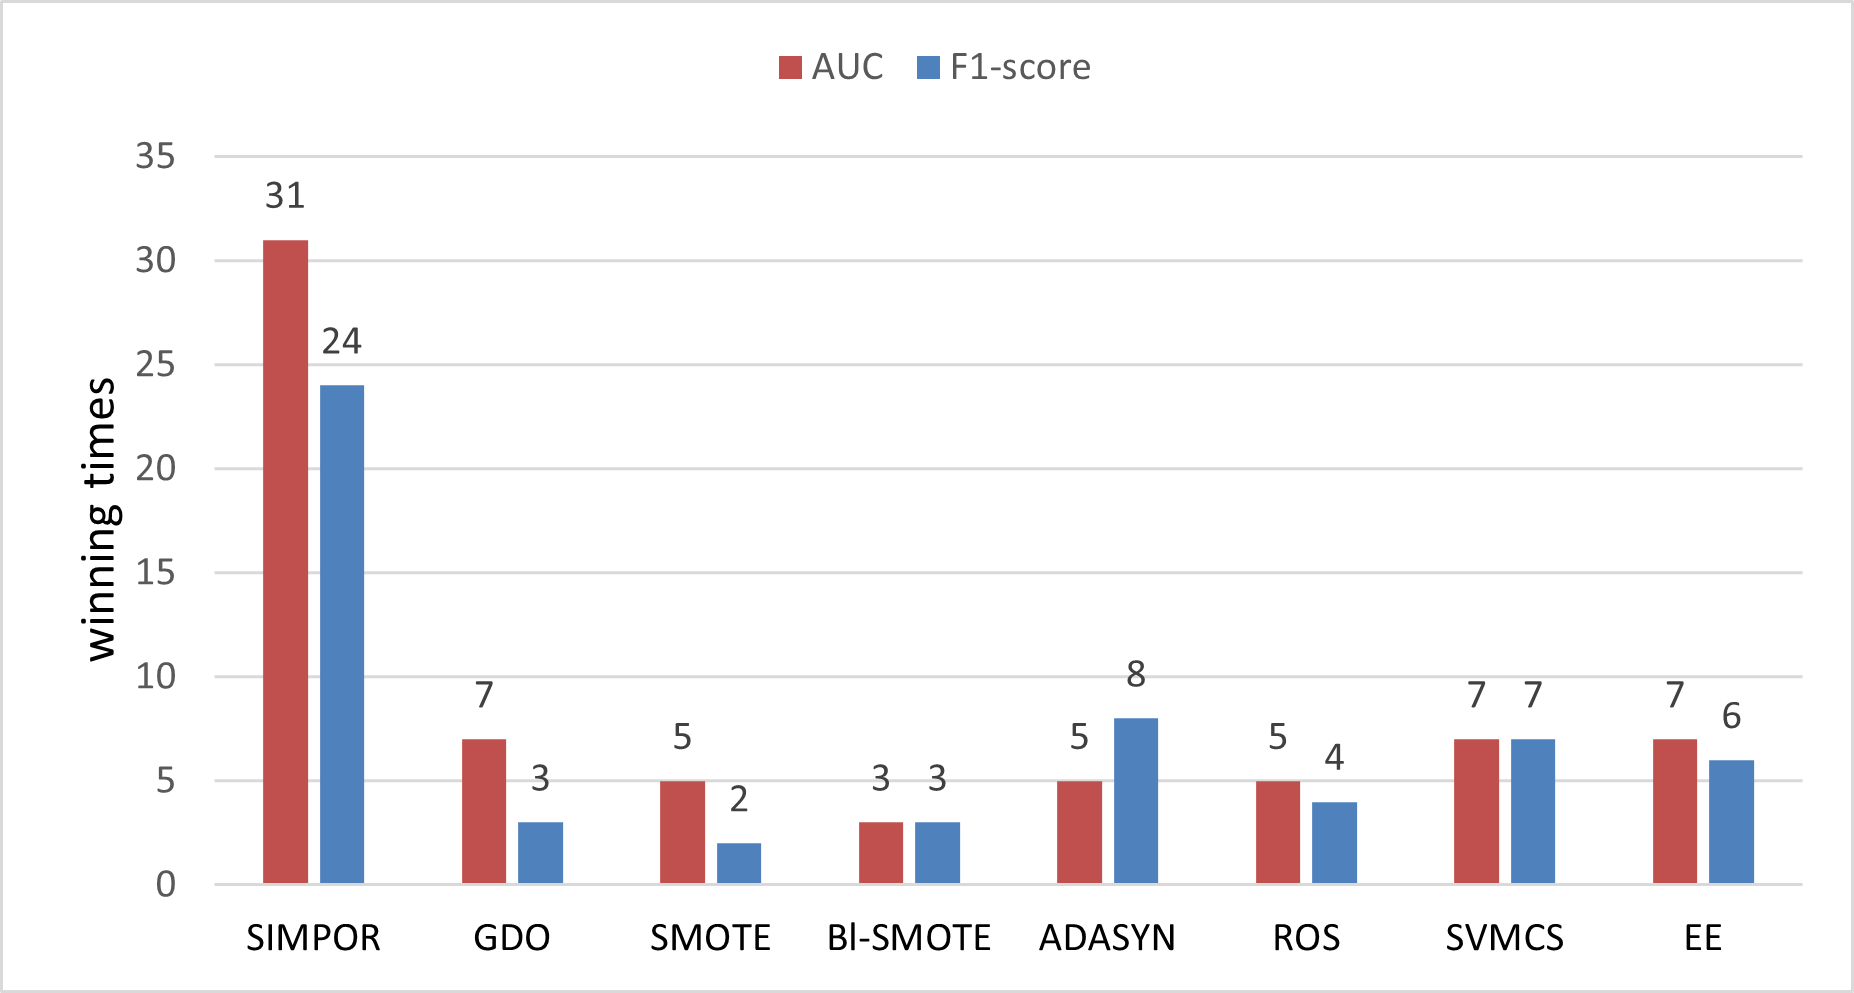
\includegraphics[width=\linewidth ]{Figures/winning_times}
	\caption{Winning times over 41 datasets.}
	\label{fig:winingTimes}
\end{figure}

Table \ref{tab:F1AllDatasets}, \ref{tab:AUCAllDatasets}, \ref{tab:Precision} and \ref{tab:Recall} show the classification F1-score, AUC, Precision, and Recall results, respectively. The highest scores for each dataset are highlighted in bold style. 
\Copy{winningTime}{We also provide the summary of the F1 and AUC scores by ``winning times" scores. We count the number of datasets for which a technique achieves the highest scores among the compared techniques and name this number ``winning times". For convention, if more than two techniques share the same highest score, the winning times will be increased for each technique. Figure \ref{fig:winingTimes} shows a summary of winning times.} 

As we can see from the table, the proposed technique outperforms others on both evaluation metrics, F1-score and AUC. More specifically, \Methodname{} hits 23 F1-score winning times and 25 AUC winning times. Its number of F1-score winning times at 23 four times better than the second winner (SVMCS) at 6, and its AUC winning times at 25 doubles the second AUC winners (EE) at 10. 


\subsection{Statistical Test.}
	\label{sec:wilcoxon}
\Copy{wilcoxonTest}{
To further evaluate the effectiveness of the technique, we also performed a Wilcoxon Signed Rank Test \cite{wilcoxon} on the 41 dataset results (F1 score and AUC). Wilcoxon hypothesis test is relevant to our study as it is a non-parametric statistical test and does not require a specific distribution assumption for the results. On the other hand, 41 data points (corresponding to 41 datasets results) are sufficient to support this test. Our null hypothesis is that the difference between the proposed technique results and those of the other technique is insignificant. Wilcoxon signed-rank test outputs are computed over the 41 dataset results and return a p-value for each technique pair. We then compare the p-value with the significant value $\alpha = 0.05$. Suppose the p-value is smaller than $\alpha$. In that case, the evidence is sufficient to reject the hypothesis, which means the proposed technique does make a significant difference from the others, and vice versa. Table \ref{tab:wilcoxonTest} shows the Wilcoxon p-value results.

	\begin{table}[htbp]
		\centering
		\caption{Wilcoxon Signed Rank Hypothesis Test results.}
		
		\begin{tabular}{lcc}
			\toprule
			& \multicolumn{2}{c}{p-value} \\
			\midrule
			SIMPOR vs. & \multicolumn{1}{l|}{F1-score} & \multicolumn{1}{l}{AUC} \\
			\midrule
			GDO   & 1.82E-03 & 1.93E-03 \\
			SMOTE & 2.66E-03 & 6.64E-05 \\
			BL\_SMOTE & 4.22E-03 & 1.63E-04 \\
			ADASYN & 2.89E-03 & 6.13E-04 \\
			DeepSM   & 6.40E-04 & 2.57E-04 \\
			SVMCS & 2.74E-03 & 3.40E-02 \\
			EE    & 1.99E-03 & 2.17E-02 \\
			\bottomrule
		\end{tabular}%
		\label{tab:wilcoxonTest}%
	\end{table}%

As we can see from Table \ref{tab:wilcoxonTest}, the p-values are all smaller than the critical value of 0.05. Thus, the null hypothesis can be rejected as the supporting evidence is sufficient. In other words, the statistical result shows that the proposed technique makes a significant improvement compared to others.     
}


\subsection{Data visualization}  

\begin{figure*}[h!]
	\centering
	%[trim=left bottom right top, clip]
	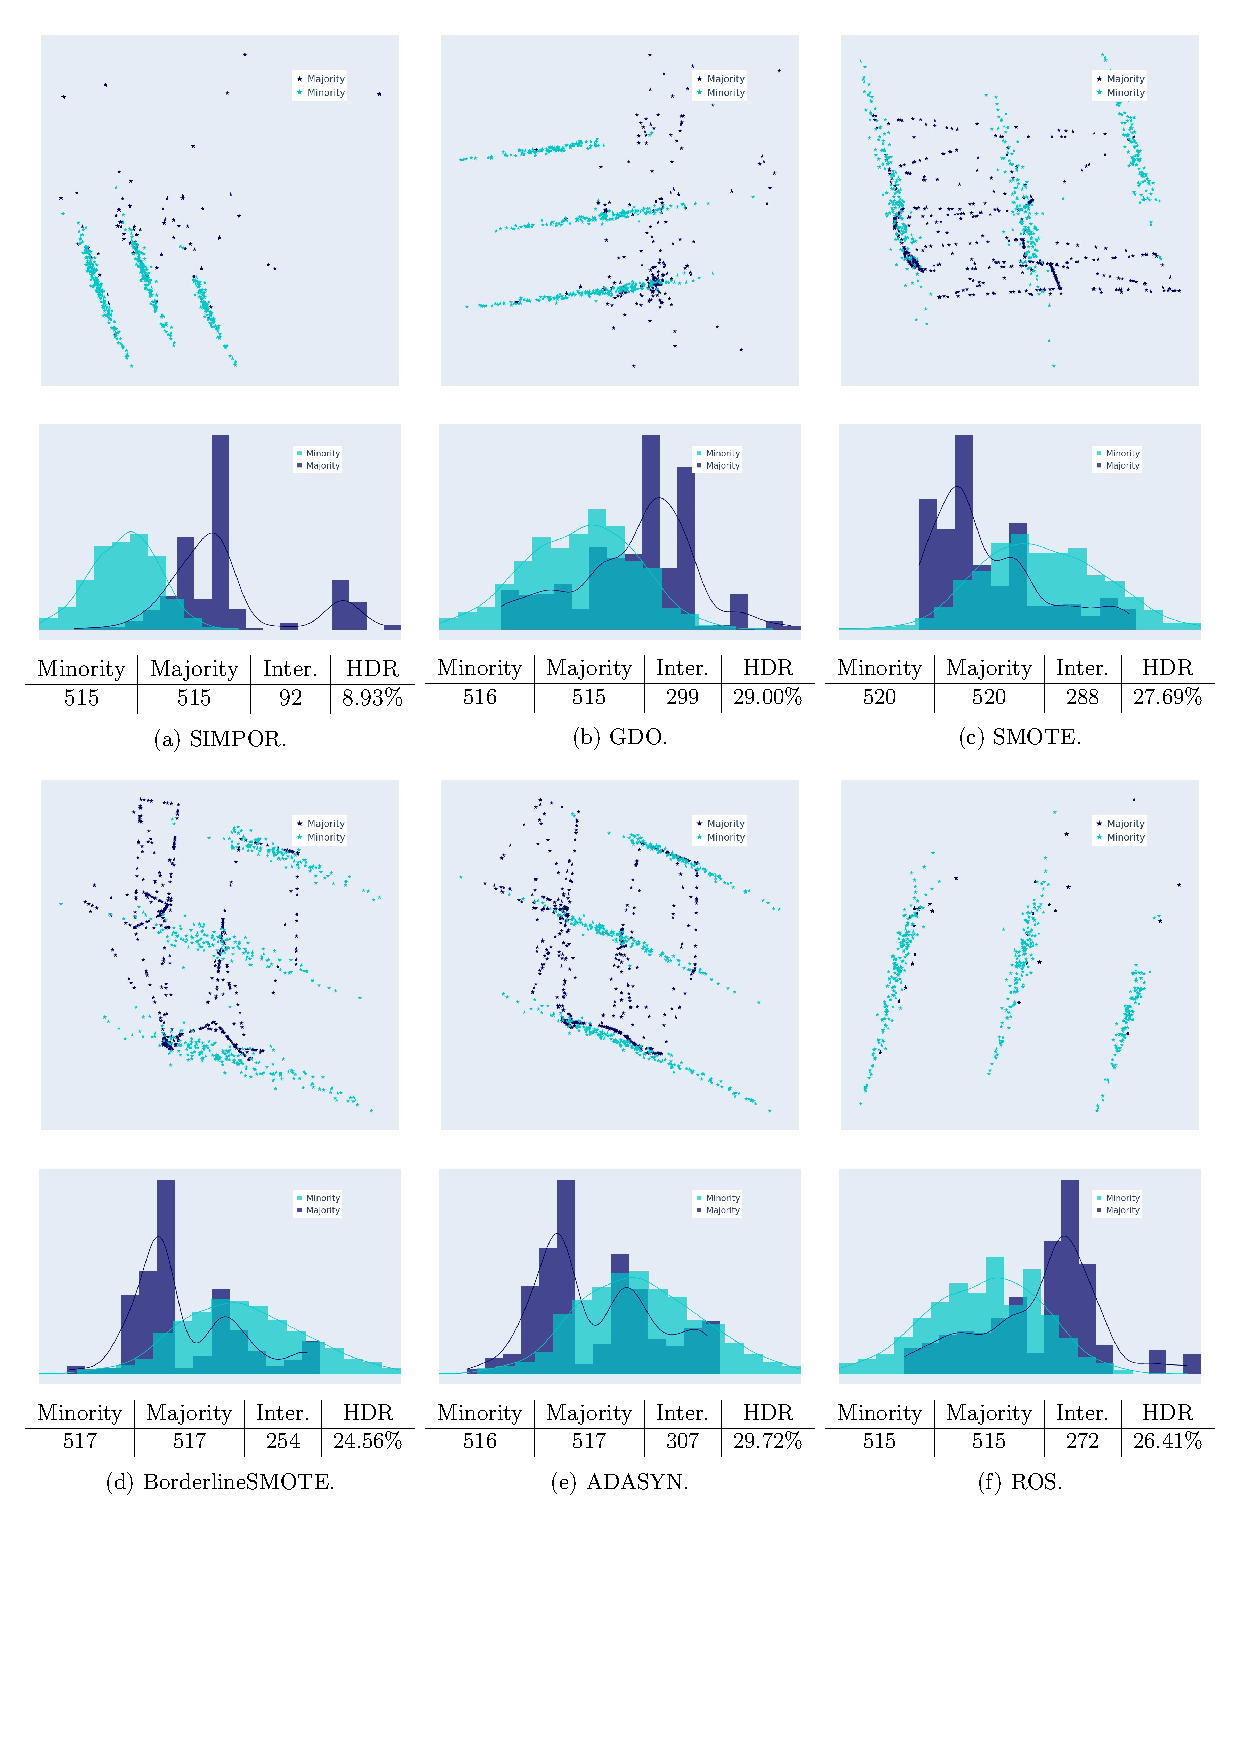
\includegraphics[width=0.8\linewidth,trim=10 90 10 10, clip ]{Figures/PCA/abalone9-18}
	\caption{Abalone9-18: Generated training data projected onto 2-dimension space and their histograms in 1-Dimension space using Principle Component Analysis dimension reduction technique. The bottom tables illustrate the number of samples in two classes, 1-Dimension histogram intersection between 2 classes, and the hard-to-differentiate ratio between the number of intersection samples to the number of minority samples ($HDR = \frac{Inter.}{Minority}100\%$).}
	\label{fig:visualization1d2d}
\end{figure*}

\R{histogramVisualization}
\Copy{histogramVisualization}{
To explore more on how the techniques perform, we visualize the generated data by projecting them onto lower dimension space (i.e., one and two dimensions) using the Principle Component Analysis technique (PCA) \cite{pca}. Data's 2-Dimension (2D) plots and 1-Dimension histograms are presented with a hard-to-differentiate ratio (HDR) for each technique. 1D histograms are computed by dividing one-dimensional-reduced data into 20 bins (intervals) and counting the number of samples within the interval of each bin. A hard-to-differentiate ratio is defined as the ratio of the number of samples in the intersection between 2 classes to the total of minority samples ($HDR = \frac{No.\: Intersection \: samples}{No. \: Minority \: samples}100\% $) where the number of intersection samples is estimated by counting samples in the overlapped bins between the two classes in the 1D histograms. This ratio is expected to be as small as 0\% if the two classes are well separated; in contrast, 100\% indicates that the two classes cannot be distinguished in the projected 1D space. Besides HDR, we show the absolute numbers of Minority, Majority, and Intersection samples for each technique in the bottom tables. From the plots, we observe how the data are distributed in 2D space and quantify samples that are hard to be differentiated in the 1D space histograms.       
}

To save space, we only show the plot of one dataset (i.e., Abalone9-18 dataset) in Figure \ref{fig:visualization1d2d}. Many other datasets are observed to have similar patterns. We observe that the proposed technique does not poorly generate synthetic samples as many as other techniques do. HDR results show that \Methodname{} achieves the least number of hard-to-differentiate ratio at 15.47\%. As shown in the 2D visualization sub-figures, other techniques poorly-place synthetic data crossed the other class. This causes by outliers or noises near the border between the two classes that other techniques do not pay attention to and mistakenly create more noise. In contrast, \Methodname{} safely produces synthetic data towards the minority class by maximizing the posterior ratio ;thus it can reduce the number of poorly-placed samples.
 
 
 
\Copy{processingTime}{ 
\begin{table}[htbp]
	\centering
	\caption{Processing time (in seconds) over 41 datasets.}
	\resizebox{0.97\columnwidth}{!}{%
		
	    \begin{tabular}{lcccccc}
	    	\toprule
	    	& SIMPOR & GDO   & SMOTE & BL-SMOTE & ADASYN & DeepSM \\
	    	\midrule
	    	glass1 & 0.1147 & 0.0576 & 0.0020 & 0.0033 & 0.0032 & 0.8587 \\
	    	wisconsin & 2.0805 & 0.1769 & 0.0024 & 0.0044 & 0.0046 & 1.2004 \\
	    	pima  & 0.2032 & 0.2066 & 0.0025 & 0.0049 & 0.0050 & 1.2297 \\
	    	glass0 & 0.2157 & 0.0553 & 0.0023 & 0.0035 & 0.0036 & 0.8601 \\
	    	yeast1 & 0.2457 & 0.4749 & 0.0035 & 0.0108 & 0.0104 & 1.4846 \\
	    	haberman & 0.0517 & 0.1560 & 0.0022 & 0.0033 & 0.0036 & 0.9246 \\
	    	vehicle1 & 0.4365 & 0.1237 & 0.0025 & 0.0059 & 0.0059 & 1.4147 \\
	    	vehicle2 & 6.2913 & 0.1512 & 0.0029 & 0.0053 & 0.0061 & 1.3976 \\
	    	vehicle3 & 0.2821 & 0.1237 & 0.0024 & 0.0060 & 0.0061 & 1.3487 \\
	    	creditcard & 2.1200 & 0.3783 & 0.0087 & 0.0184 & 0.0182 & 1.7980 \\
	    	glass-0-1-2-3\_vs\_4-5-6 & 0.3376 & 0.0459 & 0.0023 & 0.0035 & 0.0035 & 0.8407 \\
	    	vehicle0 & 7.3645 & 0.1198 & 0.0024 & 0.0054 & 0.0058 & 1.2953 \\
	    	ecoli1 & 0.0418 & 0.0337 & 0.0010 & 0.0018 & 0.0017 & 0.9310 \\
	    	new-thyroid1 & 0.5352 & 0.0304 & 0.0015 & 0.0024 & 0.0024 & 0.8590 \\
	    	new-thyroid2 & 0.3881 & 0.0359 & 0.0025 & 0.0033 & 0.0031 & 0.8747 \\
	    	ecoli2 & 0.2516 & 0.0266 & 0.0011 & 0.0017 & 0.0016 & 0.9733 \\
	    	glass6 & 0.3196 & 0.0268 & 0.0014 & 0.0025 & 0.0023 & 1.0744 \\
	    	yeast3 & 0.1374 & 0.2422 & 0.0023 & 0.0060 & 0.0059 & 1.6699 \\
	    	ecoli3 & 0.0658 & 0.0378 & 0.0015 & 0.0025 & 0.0024 & 0.9647 \\
	    	page-blocks0 & 7.9654 & 2.0918 & 0.0045 & 0.0143 & 0.0138 & 3.6029 \\
	    	yeast-2\_vs\_4 & 2.4310 & 0.0624 & 0.0017 & 0.0028 & 0.0028 & 1.0286 \\
	    	yeast-0-5-6-7-9\_vs\_4 & 0.0868 & 0.0632 & 0.0016 & 0.0029 & 0.0027 & 0.9809 \\
	    	vowel0 & 4.7675 & 0.1312 & 0.0018 & 0.0039 & 0.0037 & 1.2410 \\
	    	glass-0-1-6\_vs\_2 & 0.0482 & 0.0207 & 0.0013 & 0.0023 & 0.0022 & 0.9133 \\
	    	glass2 & 0.0501 & 0.0227 & 0.0013 & 0.0024 & 0.0024 & 0.8855 \\
	    	yeast-1\_vs\_7 & 0.4697 & 0.0420 & 0.0017 & 0.0026 & 0.0026 & 1.0355 \\
	    	glass4 & 0.1141 & 0.0197 & 0.0012 & 0.0024 & 0.0023 & 0.9469 \\
	    	ecoli4 & 0.1087 & 0.0310 & 0.0015 & 0.0024 & 0.0024 & 0.9393 \\
	    	page-blocks-1-3\_vs\_4 & 1.8742 & 0.0445 & 0.0015 & 0.0027 & 0.0026 & 0.9992 \\
	    	abalone9-18 & 2.9722 & 0.0716 & 0.0015 & 0.0028 & 0.0026 & 1.2095 \\
	    	yeast-1-4-5-8\_vs\_7 & 0.0881 & 0.0673 & 0.0017 & 0.0031 & 0.0028 & 1.0803 \\
	    	glass5 & 0.2815 & 0.0241 & 0.0017 & 0.0033 & 0.0036 & 0.8550 \\
	    	yeast-2\_vs\_8 & 0.1239 & 0.0441 & 0.0016 & 0.0027 & 0.0028 & 0.9849 \\
	    	car\_eval\_4 & 0.4381 & 0.1746 & 0.0026 & 0.0066 & 0.0049 & 1.6616 \\
	    	wine\_quality & 0.1622 & 0.8587 & 0.0030 & 0.0144 & 0.0137 & 3.3128 \\
	    	yeast\_me2 & 0.1060 & 0.1379 & 0.0018 & 0.0042 & 0.0039 & 1.7350 \\
	    	yeast4 & 0.1083 & 0.1386 & 0.0018 & 0.0041 & 0.0039 & 1.6314 \\
	    	yeast-1-2-8-9\_vs\_7 & 0.0924 & 0.0757 & 0.0017 & 0.0031 & 0.0030 & 1.3069 \\
	    	yeast5 & 0.1188 & 0.1312 & 0.0019 & 0.0037 & 0.0040 & 1.6181 \\
	    	yeast6 & 0.0613 & 0.1419 & 0.0018 & 0.0037 & 0.0036 & 1.6382 \\
	    	abalone19 & 0.0890 & 0.3161 & 0.0022 & 0.0053 & 0.0054 & 3.0168 \\
	    	\bottomrule
	    \end{tabular}%
		
	}
	\label{tab:ProcessingTime}%
\end{table}%

\subsection{Processing Time.}
\label{sec:processingTime}
Data processing times for oversampling-based approaches on 41 datasets are compared to provide a more comprehensive comparison. We don't compare them to the other approaches, i.e., cost-sensitive learning and ensemble learning, because they only need negligible data processing time as they focus on classifiers other than improving the data. The processing time was recorded from our machine, which uses an Intel i7 32-thread processor and two NVIDIA 3090 Ti GPUs. 
Table \ref{tab:ProcessingTime} shows the recorded processing time over 41 datasets. Overall, our technique takes longer than others as we have to compute the kernel estimation for each data point, as mentioned in Section \ref{sec:implementation}. Similarly, DeepSMOTE generally suffers high time consuming cost because it heavily relies on underlying heuristic methods. In other words, the proposed technique is slower, but it provides better F1 and AUC scores than others.

}

\begin{figure*}[ht]
	\centering
	%[trim=left bottom right top, clip]
	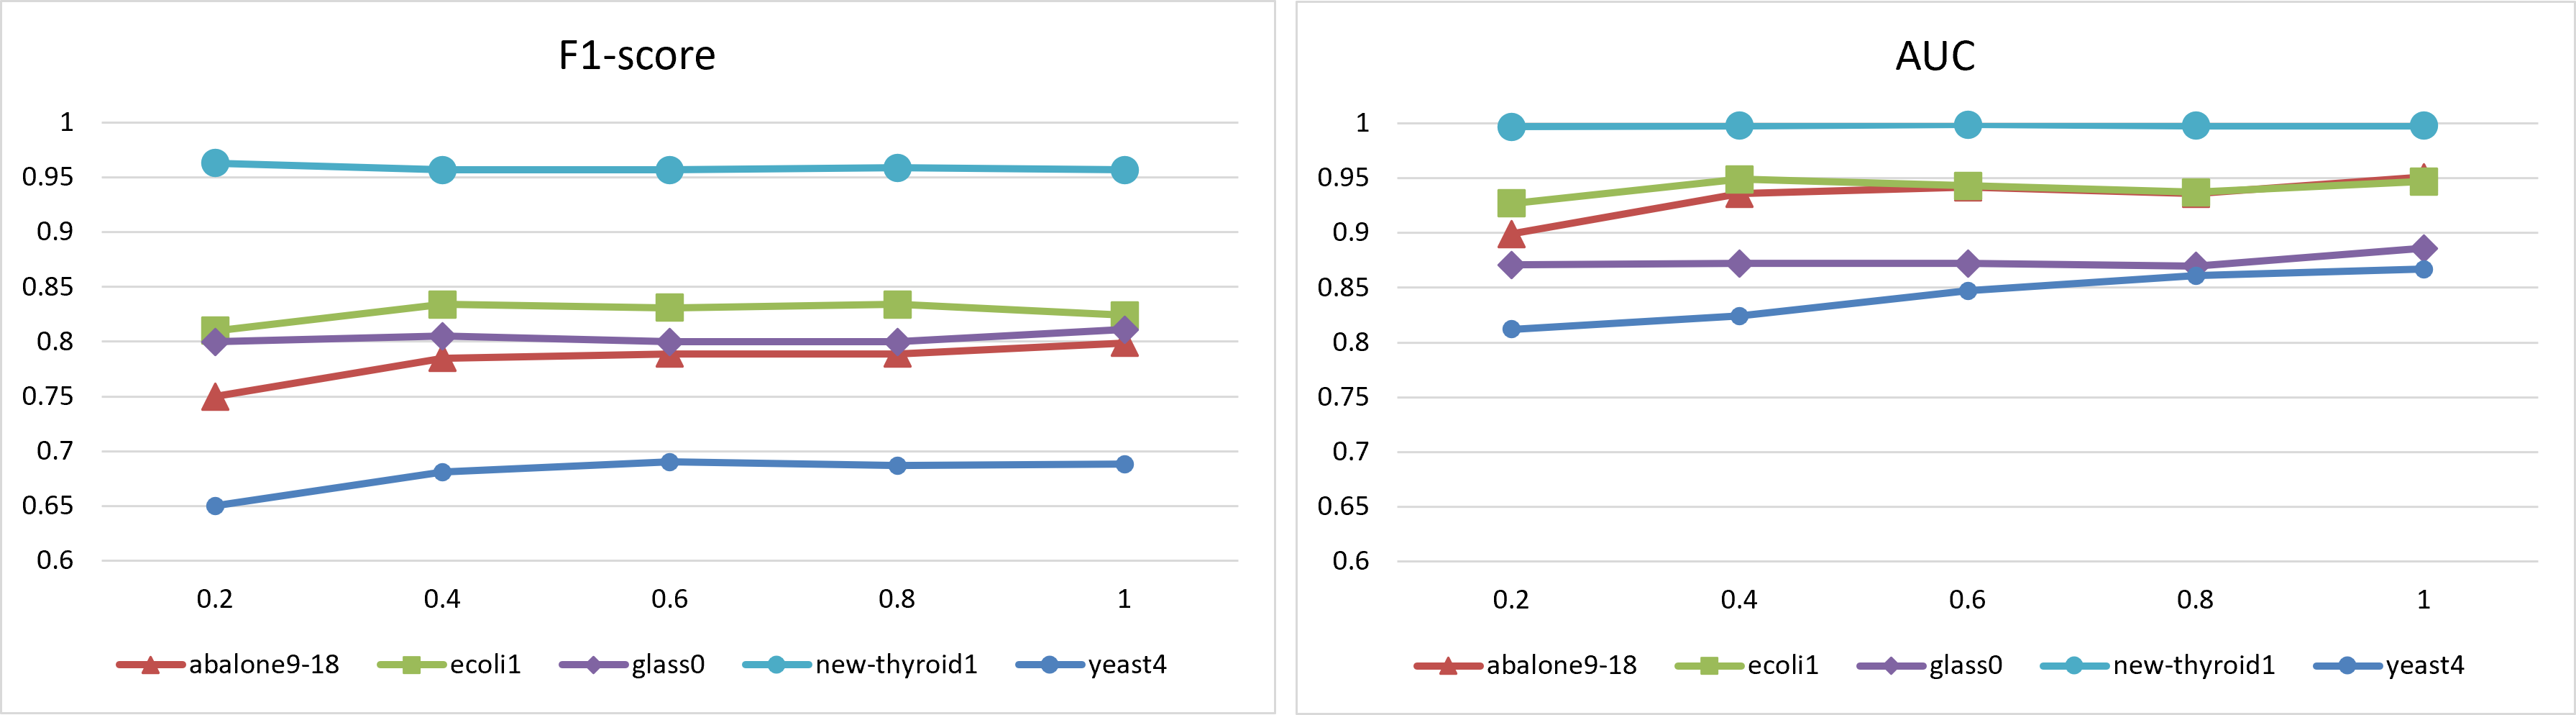
\includegraphics[width=0.98\linewidth, trim=5 10 10 10, clip ]{Figures/r_impact}
	\caption{F1-score and AUC results with varying Gaussian standard deviation (ranging from 0.2R to R).}
	\label{fig:r_result}
\end{figure*}

\begin{figure*}[h]
	\centering
	%[trim=left bottom right top, clip]
	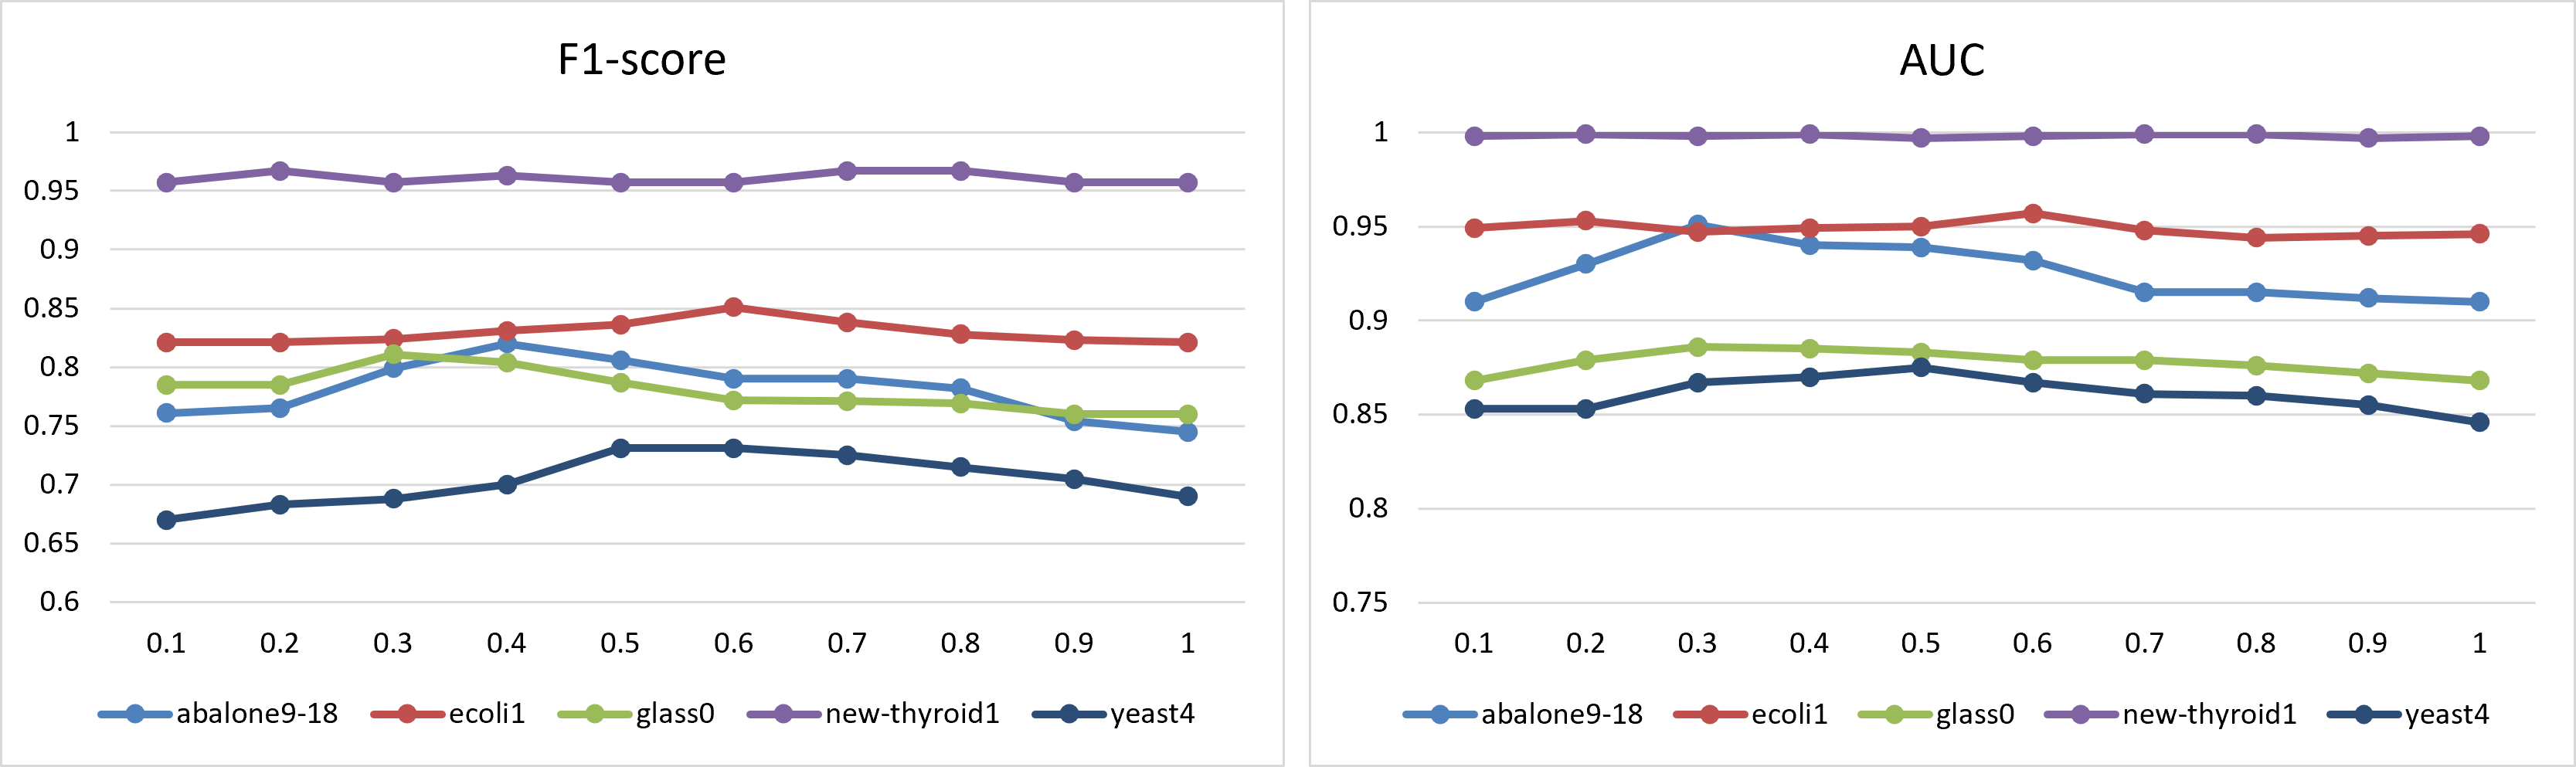
\includegraphics[width=0.98\linewidth, trim=5 10 10 10, clip ]{Figures/threshold_impact}
	\caption{F1-score and AUC results with varying informative portion IP.}
	\label{fig:ip_result}
\end{figure*}

\subsection{Empirical study on the impact of radius factor r.}
\label{sec:simpor_r_distribution_impact}
In this section, we study how the classification performance is impacted by different generation radius factor $r$ in Equation \ref{equ:r_dist}. The classification performance is measured under different distribution settings of the radius r as it controls how far synthetic data are generated from its original minority sample. We use different parameters for the Gaussian distribution $\mathcal{N}(\mu ,\,{(\alpha R)}^{2})$. Particularly, we fix the mean value to zero and change $\alpha$ from 0.2 to 1 with steps of 0.2 so that the Gaussian standard deviation $\alpha R$ will range from 0.2R to R. To save space, we arbitrarily select 5 datasets to conduct this experiment. The classification results are shown in Figure \ref{fig:r_result}. 

\R{EmpiricalExplanation}
\Copy{EmpiricalExplanation}{
The figure obtained from the experiment indicates that the r factor, with a radius distribution standard deviation ranging from 0.6R to R, has minimal impact on the classification performance. While there are slight variations within the $\alpha$ range of 0.6 to 1, the performance improves between 0.2 to 0.6 (such as for ecoli1, abalone9-18, and yeast4). This is because the performance mainly depends on the classifier's decision boundary, and the synthetic data are placed far away from the decision boundary towards the minority class area; thus,  the radius does not have much effect on the accuracy results. However, in the case of multi-classed data, the performance might be affected by a significant value of R. 
}
\subsection{Empirical study on the impact of informative portion (IP).}
This section studies the empirical impact of the informative portion (IP) in Section \ref{sec:EAL}. This portion works as a threshold to adjust how many samples are taken into consideration of informative samples. To save space, we study five datasets used in Section \ref{sec:simpor_r_distribution_impact}. Different values of IP ranging from 0.1 to 1 are applied, and the classification performance results are shown in Figure \ref{fig:ip_result}.

\R{EmpiricalExplanationIP}
\Copy{EmpiricalExplanationIP}{
As we can see from the figure, while datasets with outstanding performance (new-thyroid1, ecoli1) have little impact, there are fluctuations in other datasets' F1-score and AUC score  (abalonce9-18, glass0, yeast4). This is because, for the easy-separated dataset such as new-thyroid1 and ecoli1, the IP change does not affect the classification performance as the data classes are easily separated. While in more challenging datasets, IP changes might affect the balance at the informative region; thus, this leads to performance variations. The resulting figure also suggests tuning IP for each dataset between a range of (0.2, 0.6) could achieve higher performance.
}







	
	
\section{Related Work}
\label{sec:relatedwork}
In the last few decades, there have been a number of solutions proposed to alleviate the negative impacts of data imbalance in machine learning. However, many of them are not efficient when it comes to high-dimensional data and deep learning. In this section, we review algorithms that aim at deep learning and strategies inherited from conventional machine learning methods. These techniques can mainly be categorized into two different categories, i.e., data-centric and model-centric approaches. 


Model-centric approaches usually require modifications of algorithms on the cost functions in order to balance the weight of each class. Specifically, such cost-sensitive approaches put higher penalties on majority classes and less on minority classes to balance their contribution to the final cost. For example,  \cite{cui_class-balanced_2019} provided their designed formula $ (1 - \beta^n)/(1 - \beta)$ to compute the weight of each class based on the effective number of samples $n$ and a hyperparameter $\beta$ which is then applied to re-balance the loss of a convolutional neural network model.  \cite{huang_learning_2016},\cite{rangarajan_sridhar_unsupervised_2015}, \cite{DBLP:journals/corr/abs-1805-00932} assign classes' weights inversely proportional to sample frequency appearing in each class.      


Compared to model-centric-based manners, data-centric approaches have been attracting more research attention as it is independent of machine learning algorithms. In this category, we divide into two main approaches, i.e. sampling-based and generative approaches. Sampling-based methods \cite{DBLP:journals/corr/ShenLH15}, \cite{DBLP:journals/corr/abs-1711-00941}, \cite{haibo_he_learning_2009}, \cite{li_entropy-based_2020}, \cite{ertekin_active_2007} mainly generate a balanced dataset by either over-sampling minority classes or down-sampling majority classes. Some methods are not designed for deep learning, but we still consider them since they are independent of the machine learning model architecture. In a widely used method SMOTE \cite{chawla_smote:_2002}, Chawla \textit{et al.} attempt to oversampling minority class samples by connecting an sample to its neighbors in feature space and arbitrarily drawing synthetic samples along the connections. However, one of the drawbacks of SMOTE is that if there are samples in the minority class located in the majority class, it creates synthetic sample bridges towards the majority class \cite{goswami_class_2020}. This renders difficulties in differentiation between the two classes. Another SMOTE-based work namely Borderline-SMOTE \cite{bordersmote} was proposed in which its method aims to do SMOTE with only samples near the border between classes. The samples near the border are determined by the labels of its \textit{k} distance-based neighbors (if more than half of neighbors belong to the other class, the sample is considered to be on the border). This "border" idea is similar to ours to some degree. However, finding a good \textit{k} is critical, and it is usually highly data-dependent. In addition, Borderline-SMOTE again faces the problems of SMOTE. 


Under the down-sampling category, other works \cite{ertekin_learning_2007}, \cite{aggarwal_active_2020} leverage active learning techniques to find informative samples which authors believe the imbalance ratio in these areas is much smaller than that in the entire dataset. They then classify this small pool of samples to improve the performance and expedite the training process for the SVM-based method. however, this method was only designed for SVM-based methods which mainly depend on the support vectors. Also, this potentially discards important information of the entire dataset because only a small pool of data is used.  

Generative approaches which generate synthetic samples in minor classes by sampling from data distribution are becoming more attractive as they are outperforming other methods in high dimensional data \cite{DBLP:conf/dmin/LiuGM07}. When it comes to images, a number of deep learning generative-based methods have been proposed as deep learning is capable of capturing good image representations. \cite{rashid_convergence_2012} \cite{dai_generative_2019} \cite{mullick_generative_2019} utilized Variational Autoencoder as a generative model to arbitrarily generate images from learned distributions. However, most of them assumed simple prior distributions such as Gaussian for minor classes, they tend to simplify data distribution and might not succeed in sophisticated distributions. Our solution also falls into this category; however, we leverage the idea of a mixture model to tackle this issue for image data.     
	
	\section {Conclusion}
	\label{sec:conclusion}
	We propose a data balancing technique by generating synthetic data for minority samples, which maximizes the posterior ratio to embrace the chance they fall into the minority class and do not fall across the expected decision boundary. While maximizing the posterior ratio, we use kernel density estimation to estimate the likelihood so that it is able to work with complex distribution data without requiring data distribution assumptions. In addition, our technique leverage entropy-based active learning to find and balance the most informative samples. This is important to improve model performance as we have shown in our experiments. In future work, we would like to investigate imbalanced image datasets and enhance our technique to adapt to image data.     
	
	\section*{Acknowledgment}
	
	Efforts sponsored in whole or in part by United States Special Operations Command (USSOCOM), under Partnership Intermediary Agreement No. H92222-15-3-0001-01. The U.S. Government is authorized to reproduce and distribute reprints for Government purposes notwithstanding any copyright notation thereon.  
	{\footnote{ The views and conclusions contained herein are those of the authors and should not be interpreted as necessarily representing the official policies or endorsements, either expressed or implied, of the United States Special Operations Command.} }
	
	%\balance
	
	\bibliography{citation}{}
	\bibliographystyle{plain}
		
	
	
	
\end{document}
